

\begin{figure}[!t]
    \centering
    % \vspace{-2em}
    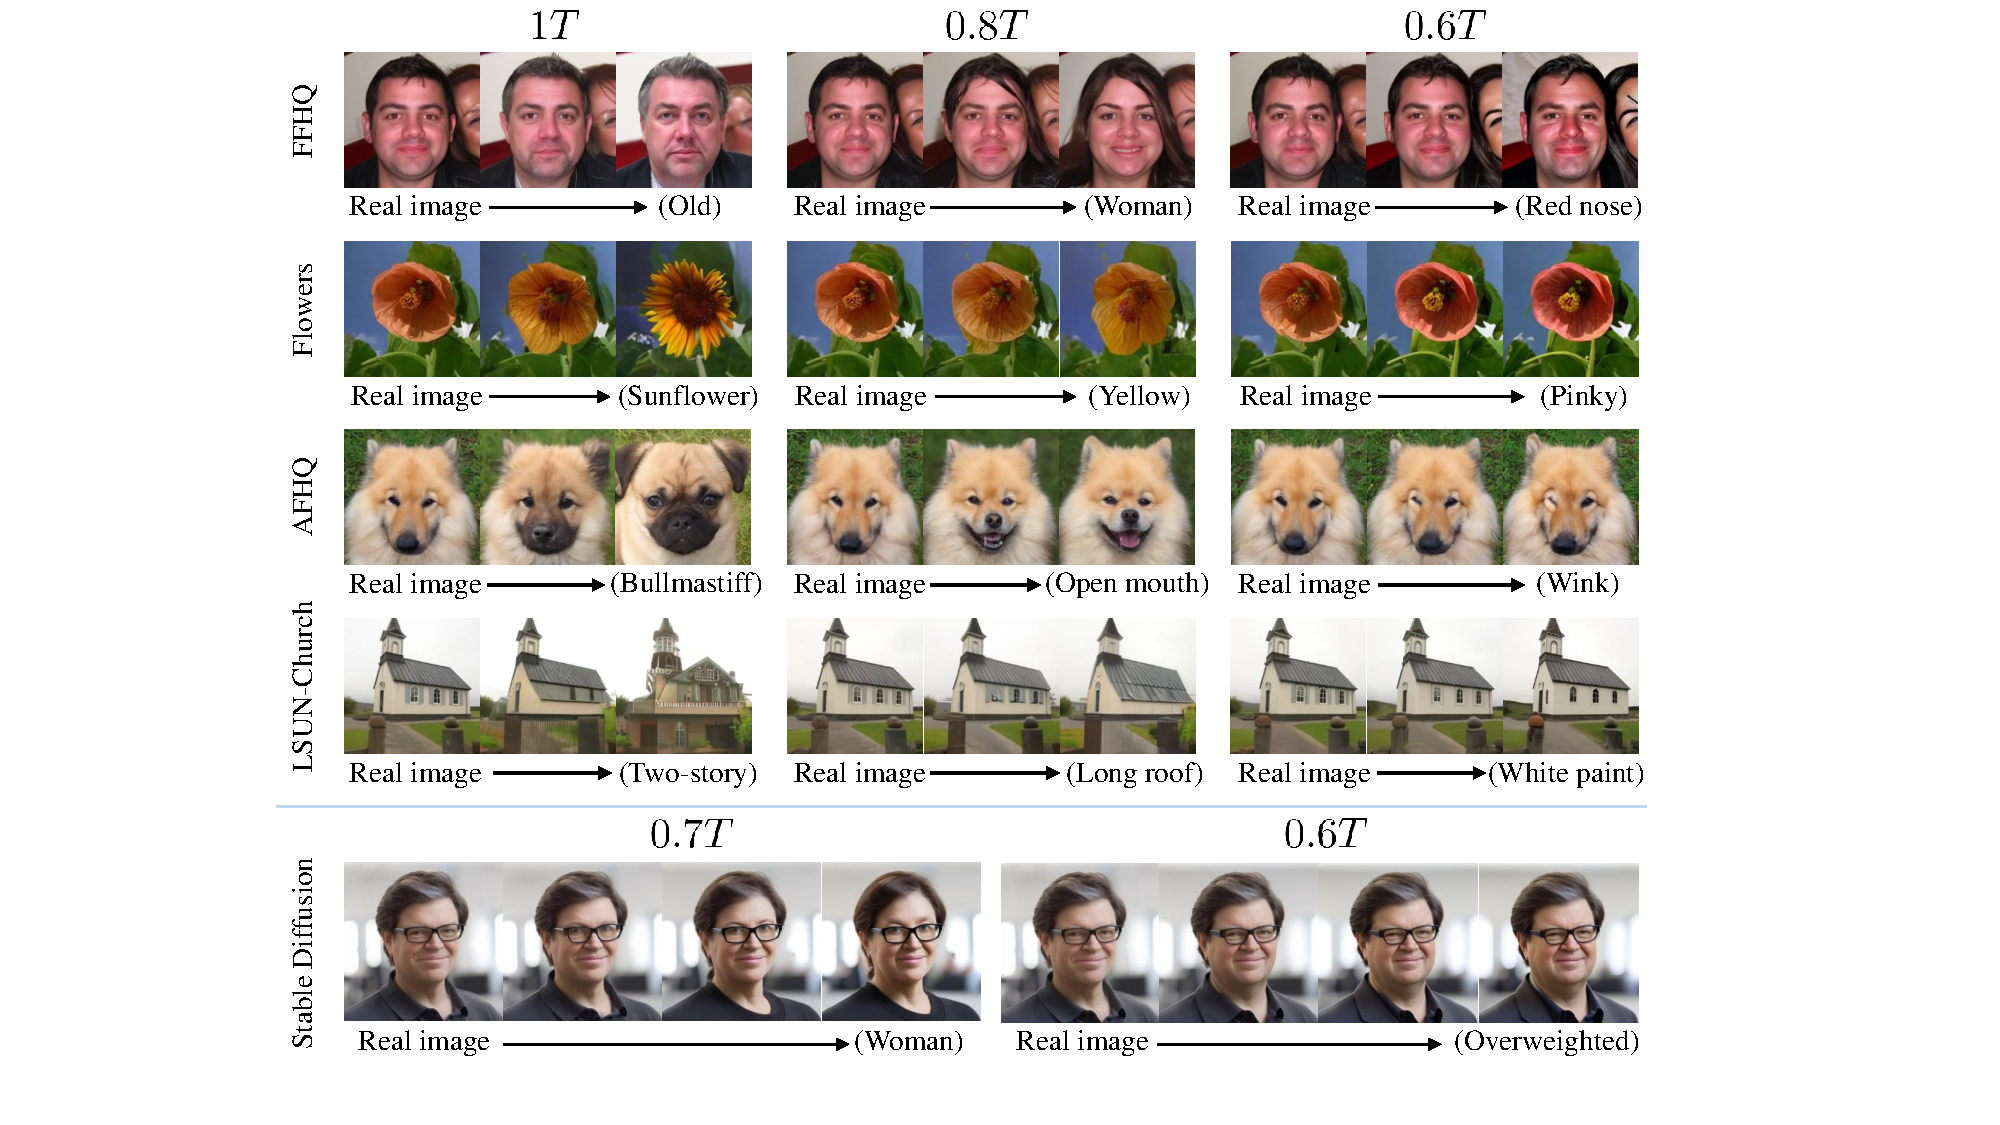
\includegraphics[width=1.0\linewidth]{figure/local_main.pdf}
    \vspace{-1em}
    \caption{\textbf{{Examples of image edition using the latent basis}.} 
    The attributes are manually interpreted {since the editing directions are not intentionally supervised.}
    For Stable Diffusion, we {used} an empty string as a prompt.
    {Each column represents edits made} at different diffusion timesteps ($0.6T$, $0.8T$, and $T$ for the unconditional diffusion model; $0.6T$ and $0.7T$ for Stable Diffusion).
    }
    \vspace{-1em}
    \label{fig:local_basis}
\end{figure}


\begin{figure}[!t]
    \centering
    % \vspace{-1.0em}
    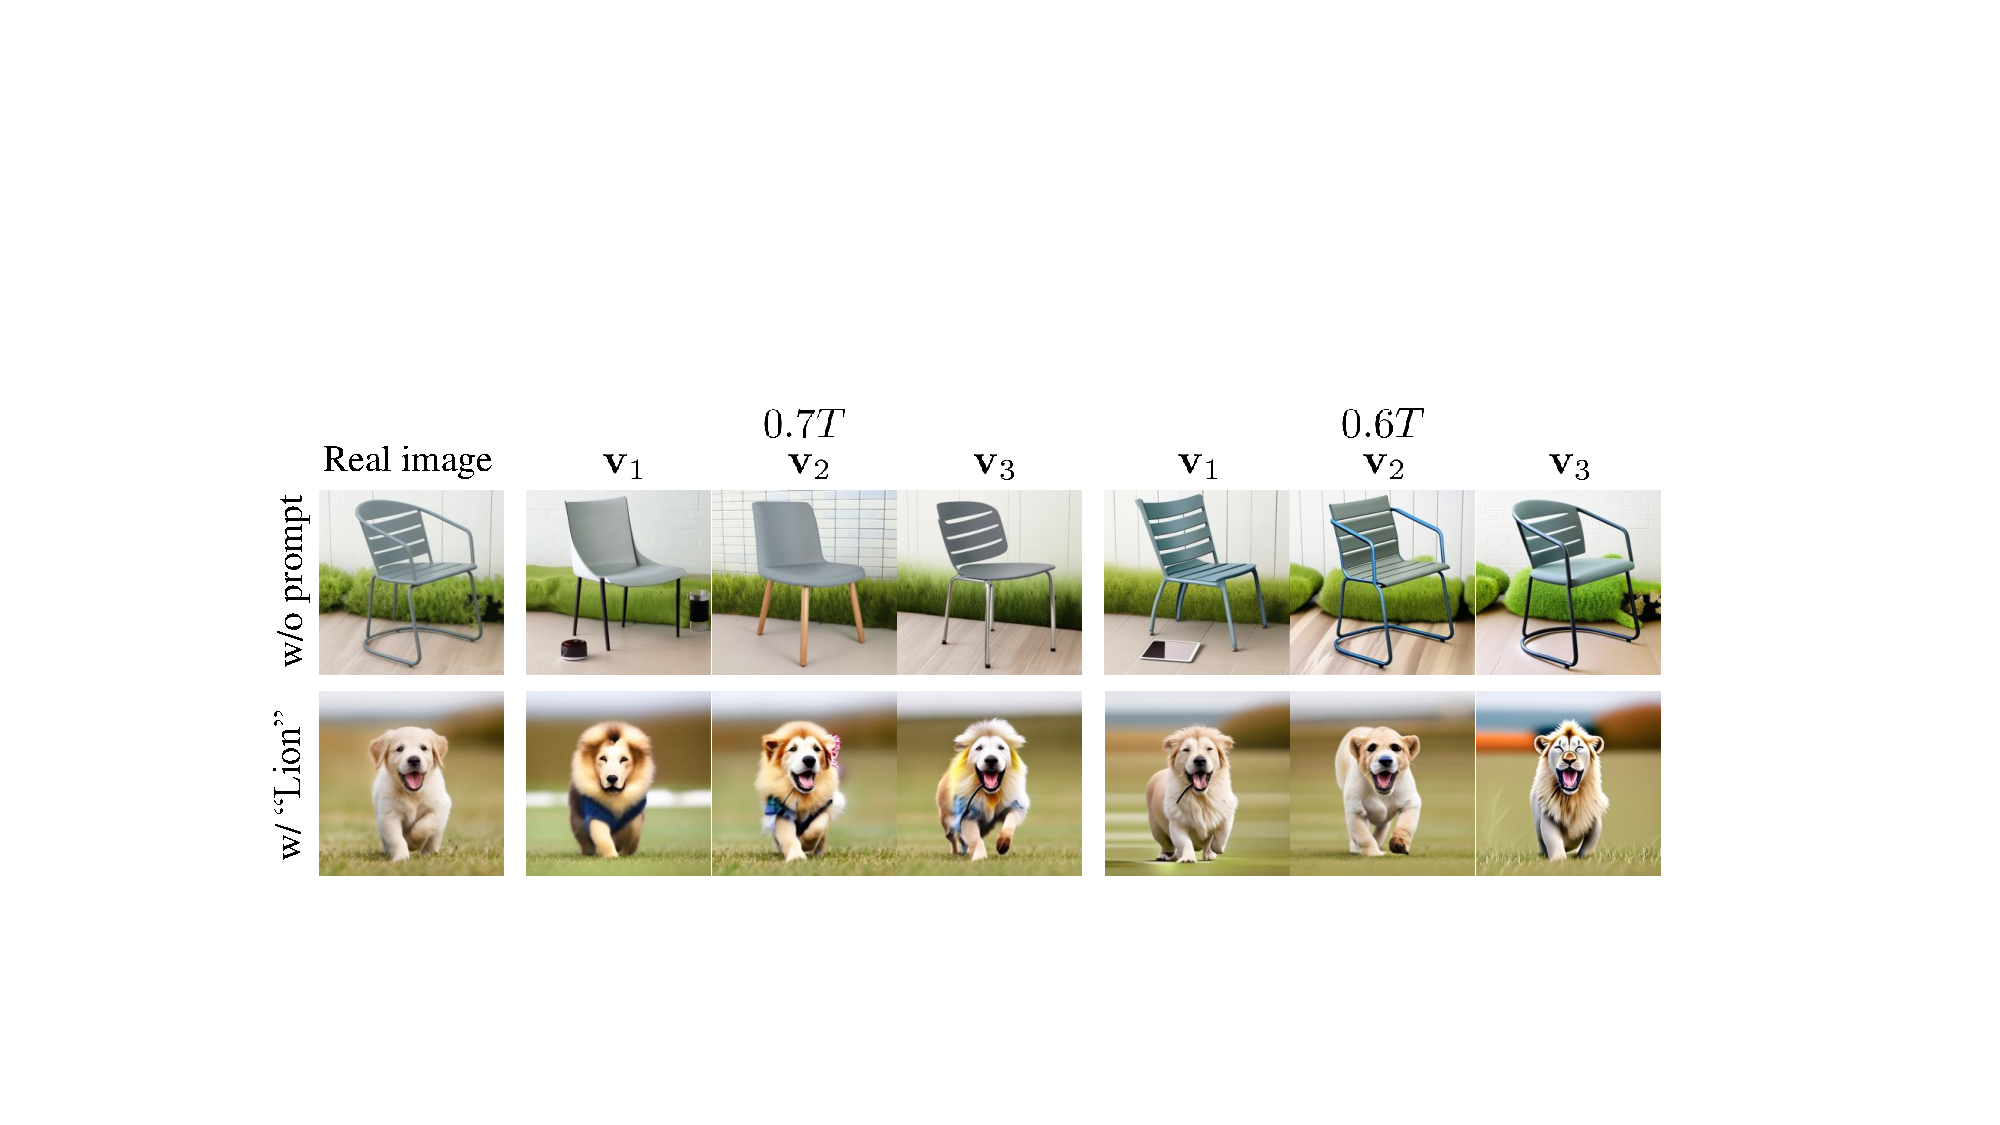
\includegraphics[width=1\linewidth]{figure/given_text_vk.pdf}
    \vspace{-1.5em}
    \caption{
    \textbf{{Examples of image edition using top-3 latent basis vectors.}} 
    {Each column is edited using a} different latent vector 
    $\{ \vv_1, \vv_2, \vv_3\}$. % are the results of manipulating the top three latent basis vectors, respectively. 
    Each group of columns {represents edits made} at different diffusion timesteps ($0.6T$ and $0.7T$).
    {Notably, when} given the ``Lion" prompt, {it is evident that all the top latent basis vectors align with the direction of the prompt.}
    %we can see that the top latent basis vectors all point in the direction of the prompt.
    }
    \vspace{-0.5em}
    \label{fig:local_basis_text_vk}
\end{figure}

\begin{figure}[!t]
    \centering
    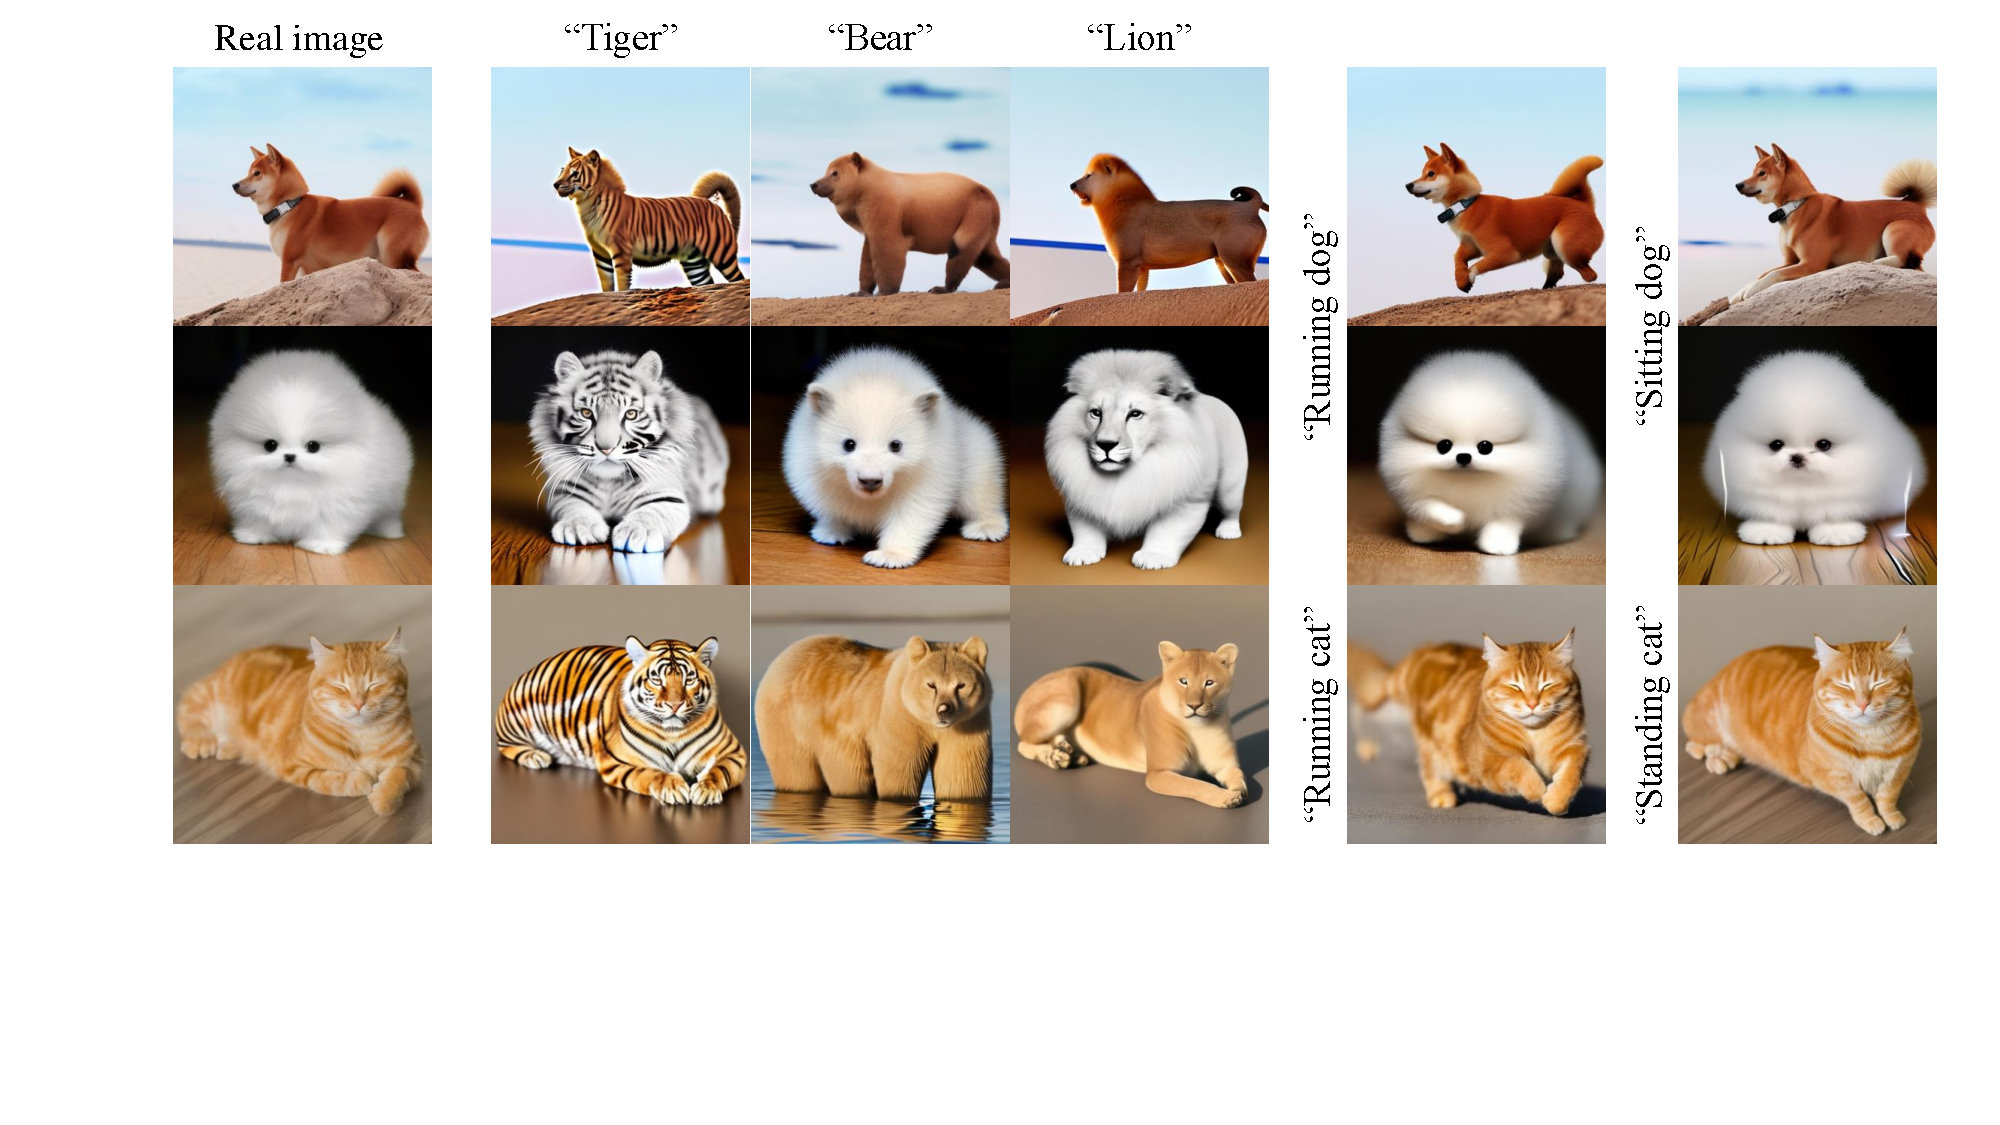
\includegraphics[width=1\linewidth]{figure/local_text_main.pdf}
    \vspace{-1.5em}
    \caption{\textbf{Examples of image edition using latent basis vectors discovered with various prompts.}
    {Each column is edited using the latent basis vector obtained from a different text prompt. Importantly, our method employs each prompt only once to derive the local latent basis.}
    %Different columns are edited by the latent basis vector found given a different text. It is worth noting that our method only uses a prompt once to get the local latent basis.
    % when manipulates the latent variable $\vx_t$.
    % \modify{샘플링할때 텍스트 영향은 아예 없는거고, 이에대한 설명 좀만 추가.}
    }
    \vspace{-1em}
    \label{fig:local_basis_text}
\end{figure}

\section{Findings and results}
In this section, we analyze the geometric structure of DMs with our method.
% In \sref{sec:local}, we demonstrate the potential of the local latent basis for real image editing.
\sref{sec:local} demonstrates that the latent basis found by our method can be used for image editing.
% In \sref{sec:local}, we validate our method by demonstrating the potential of the latent basis for real image editing.
In \sref{sec:evolution}, we investigate how the geometric structure of DMs evolves as the generative process progresses. 
% \textcircled{\raisebox{-0.9pt}{1}} The frequency domain of local latent basis changes from coarse to fine feature as the generative process progresses. % (\sref{sec:evolution-x})
% \textcircled{\raisebox{-0.9pt}{2}} The differences of local tangent spaces from various samples getting larger as the generative process progresses. % and show the possibility of parallel transport on a local basis. (\sref{sec:evolution-samples})
% \textcircled{\raisebox{-0.9pt}{3}} The differences of local tangent spaces from various timesteps depends on the complexity of the dataset.
%Lastly, in \sref{sec:text}, we discover that the geometric structure the geometric properties of the text-condition model change with a given text. % is provided.
Lastly, in \sref{sec:text}, we examine how the geometric properties of the text-condition model change with a given text. % is provided.



{The implementation details of our work are provided on \aref{appendix:implementation_detail}}. The source code for our experiments is included in the supplementary materials and will be publicly available upon publication.

%%% Move to Appendix
% \paragraph{Implementation details}
% We validated our method and provided analyses on several datasets, including ImageNet~\cite{deng2009imagenet}, LSUN-church/bedroom/cat/horse~\cite{yu2015lsun}, and CelebA-HQ~\cite{karras2018progressive} for DDPM~\cite{ho2020denoising}; and FFHQ~\cite{karras2019style}, Flowers~\cite{yu2015lsun} and AFHQ~\cite{choi2020stargan} for DDPM trained with P2 weighting~\cite{choi2022perception}. We also use Stable Diffusion (SD) version 2.1~\cite{rombach2022high} for the text-conditional diffusion model.
% For image editing, we use the official codes and pre-trained checkpoints for all baselines and keep the parameters \textit{frozen}. 
% The source code for our experiments is included in the supplementary materials and will be publicly available upon publication.

% \yh{
% Thorough experiments demonstrate the usefulness of our method in various aspects. Specifically, our approach identifies a latent basis in \exspace{}, which encompasses latent changes and exhibits a coarse-to-fine behavior, as detailed in the {\it section}. 
% Moreover, utilization of our method to Stable Diffusion allows us to investigate the effects of prompts on the local latent subspace. Our findings reveal that the impact of prompts is most pronounced at $0.7T$ and diminishes as the generative process progresses.
% }
% The latent basis in \exspace{} found by our method include latent changes and exhibit coarse-to-fine behavior {\it section}. 
% By applying our method to Stable Diffusion, we explore the impact of prompts on the local latent subspace and find that the magnitude of its impact are most significant at 0.7T and decrease as generative process progresses.
% By applying our method to Stable Diffusion, we  the latent subspace has positive correlation with the latent of \exspace{} is a spherically curved space {\it section}. Our method generalizes to stable diffusion {\it section}. Both the finding directions and the editing equation contribute to the nice properties of our method {\it section}.

%%% ICML ver
% Thorough experiments demonstrate the usefulness of our method in various aspects.
% The editing latent directions in \exspace{} found by our method include latent changes and exhibit coarse-to-fine behavior (\sref{sec:local}). \exspace{} is a spherically curved space (\sref{sec:slerp}). Our method generalizes to stable diffusion (\sref{sec:stable}). Both the finding directions and the editing equation contribute to the nice properties of our method (\sref{sec:ablation}). Our method outperforms the existing methods (\sref{sec:comparison}).

% We validate our method and provide analyzes in 
% Stable Diffusion version 2.1 ~\cite{rombach2022high},
% ImageNet, \cite{deng2009imagenet} LSUN-church, LSUN-bedroom, LSUN-cat, LSUN-horse \cite{yu2015lsun} CelebA-HQ \cite{karras2018progressive} for DDPM \cite{ho2020denoising},
% FFHQ, Flower \cite{yu2015lsun} DDPM trained with P2 weighting \cite{choi2022perception}.
% For image editing results, we only present results for LSUN-church, CelebA-HQ, and Stable Diffusion In the main paper. For more results from other datasets, please refer to the Appendix. 
% For the quantitative results, to ensure a fair comparison, we use unconditional DMs trained at the same resolution ($256^2$) and using the same scheduling (linear scheduling).
% % To minimise the impact of prompts, except when manipulating the latent variable $\vx{}_t$, we did not use any text conditions during the inversion and image generation process using DDIM. 
% For every experiments, we use the official codes and pre-trained checkpoints for all baselines and keep the parameters \textit{frozen}. Further implementation details are deferred to {\it section}.
% The source code for our experiments is included in the supplementary materials, and will be publicly available upon publication.
% We validated our method and provided analyses on several datasets, including ImageNet~\cite{deng2009imagenet}, LSUN-church/bedroom/cat/horse~\cite{yu2015lsun}, and CelebA-HQ~\cite{karras2018progressive} for DDPM~\cite{ho2020denoising}; and FFHQ~\cite{karras2019style}, Flowers~\cite{yu2015lsun} and AFHQ~\cite{choi2020stargan} for DDPM trained with P2 weighting~\cite{choi2022perception}. We also use Stable Diffusion (SD) version 2.1~\cite{rombach2022high} for the text-conditional diffusion model.
% For image editing, we use the official codes and pre-trained checkpoints for all baselines and keep the parameters \textit{frozen}. 
% \mingi{In the main paper, we present image editing results only for LSUN-church, CelebA-HQ, and SD.} For more results from other datasets, please see the Appendix.
% For the qualitative results, w
% We used unconditional DMs trained at the same resolution ($256^2$) and diffusion schedule (linear scheduling) to ensure a fair comparison. 
% For the latent variable $\vx_T$, we randomly sample from normal distribution $\mathcal{N}(0, \textbf{I})$. 
% The source code for our experiments is included in the supplementary materials and will be publicly available upon publication.



\subsection{Image editing with the latent basis}
% \subsection{\jo{latent-based editing with and without prompts}}
\label{sec:local}
% \yh{TODO : local figure 완성되고 나서 작성}

% In \sref{sec:sec3}, we introduce a method for determining local latent basis utilizing the pullback metric. 
In this subsection, we demonstrate the capability of our discovered latent basis for image editing. 
To extract the latent variables from real images for editing purposes, we use DDIM inversion.
In experiments with Stable Diffusion (SD), we do not use guidance, i.e., unconditional sampling, for both DDIM inversion and DDIM sampling processes.
This ensures that our editing results solely depend on the latent variable, not on other factors such as prompt conditions.
% This ensures that our editing result is solely the outcome of manipulating the latent variable.
% Consequently, we only utilize the text guide to extract the local latent structure and keep the generative process as unconditional sampling to minimize the influence of text.
% It is worth to note that we only use the text condition when we extract the local latent structure
% when given a text (refer to \fref{fig:text}). 

% \modify{add text conditional basis; cross attention이 특정 feature를 강조할텐데 그걸 pc를 구해도 다 텍스트에 관련된 basis만 나오는 것을 기대해야 하고, 우리가 관측한것도 이런 기대에 부합한다. text cond 피규어는 여러 local basis중에 하나 고른거고 나머지는 appendix봐라.}

Figures~\ref{fig:method} and \ref{fig:local_basis} illustrate the example results edited by the latent basis found by our method.
% demonstrate the discovery of diverse basis across different datasets which highlights the superiority of our approach \emph{without supervision} such as CLIP or a classifier. 
The latent basis clearly contains semantics such as age, gender, species, structure, and texture. 
% When modulating the strength of the basis, the resulting image undergoes continuous changes, as exemplified in \fref{fig:local_basis}. 
{Note that editing at timestep $T$ yields coarse changes such as age and species. On the other hand, editing at timestep $0.6T$ leads to fine changes, such as nose color and facial expression.} 
% Appendix provides more examples.
% In the subsequent section, we delve into a detailed analysis of the latent basis from these distinct timesteps.

% Significantly, editing at timestep $T$ results in coarse changes, whereas editing at timestep $0.6T$ produces finer changes, as exemplified by various examples. 
% In the following section, we will thoroughly explore and analyze the local semantic foundation derived from these distinct timesteps.

\fref{fig:local_basis_text_vk} demonstrates the example results edited by the various latent basis vectors.
Interestingly, using the text ``lion'' as a condition, 
the entire latent basis {captures lion-related attributes.} % aligns with the text.
% Moreover, \fref{fig:local_basis_text} shows that the latent basis can be aligned with the text not only for the type of object but also the action.
Furthermore, \fref{fig:local_basis_text} shows that the latent basis aligns with the text not only in terms of object types but also in relation to pose or action.
\modify{For a qualitative comparison with other state-of-the-art image editing methods, refer to 
\aref{appendix:comparisons}. For more examples of editing results, refer to \aref{appendix:additional_results}.}

% \fref{fig:local_basis_text_vk} demonstrates the impact on the basis of the tangent space when considering a given text. 
% One can expect the obtained basis from \ehspace{} becomes influenced by the text condition. 
% Consequently, anticipations align with our observations. 
% \modify{In the case of unconditional conditions}, the basis exhibits distinct characteristics. However, upon using the text ``lion" as a condition, noticeable lion-related modifications can be observed across all basis. This phenomenon enables editing within the semantic subspace that corresponds to the intended text, as depicted in \fref{fig:local_basis_text}. 
% We selected one of the bases, yet each basis consistently yielded results associated with the given text. It is intriguing that the capability for editing extends even to actions, such as running, even though we just added the basis only one time. Please refer to the appendix for other bases.
% In this subsection, we demonstrate our discovered latent basis through real image editing. 
% By adding the latent basis vector by utilizing the x-space guidance, we were able to apply semantic manipulations to the image.
% In Stable Diffusion, the latent basis manipulates the image in a way that is semantically aligned with the given prompt.

% \paragraph{Unconditioanl DMs}
% \yh{
% \fref{fig:local_basis} illustrates the example results edited by the directions found by our method \emph{without supervision} such as CLIP or a classifier. 
% The directions clearly contain semantics such as gender, age, ethnicity, facial expression, breed, and texture. 
% Interestingly, editing at timestep $T$ leads to coarse changes such as hair color, hair length, far breed. On the other hand, editing at the timestep $0.5T$ leads to fine changes such as make-up, hair texture, wrinkles, facial expression, and close breed. \aref{appendix:local} provides more examples.
% }\yh{
% \fref{fig:global_basis_main} demonstrates that the global directions in $\vx_t$ lead to the same semantic changes, such as rotation, age, furriness, or color in different samples. 
% It confirms that \exspace{} inherits the homogeneity of \ehspace{} via the pullback metric although \exspace{} is a metric-less space. \aref{appendix:global} provides more examples.
% }\yh{
% \paragraph{Stable Diffusion} 
% This section demonstrates that our method is generalized to Stable Diffusion \cite{rombach2022high}. Our method extracts latent directions in the learned latent space $\vz_t$ using the same procedure. \fref{fig:ldm} (a) shows the edited images along different directions on various timesteps. 
% The phenomena are similar to the image-based DMs: 
% editing at $t=T$ provides coarse changes, and editing at later timesteps provides more fine texture-ish changes such as cartoonization.
% }

% Furthermore, \fref{fig:ldm} (b) 는 prompt 가 주어지는 경우 local latent basis 를 활용한 결과를 보여주고 있다.  
% 예를 들어, jumping dog 

%%% ICML ver
% Furthermore, \fref{fig:ldm} (b) shows that a global semantic direction leads to the same \textit{zoom-out} effect on different samples. Contrary to the global directions in the image-based DMs, the global directions are found within a text prompt, i.e., each text prompt has its own global directions. \aref{appendix:additional_results} provides more examples where we find some odd cases indicating that the learned latent space may not follow the same assumptions of the image-based DMs or the text guidance somehow twists the manifold.

%%% ICML ver
% \fref{fig:global_btasis_main} demonstrates that the global directions in $\vx_t$ lead to the same semantic changes, such as roation, age, furriness, or color in different samples. It confirms that \exspace{} inherits the homogeneity of \ehspace{} via the pullback metric although \exspace{} is a metric-less space. \aref{appendix:global} provides more examples.



%\subsection{Evolution of Semantic Structure \yh{of DMs} over Timesteps.}
\subsection{{Evolution of latent structures during {generative} processes}}
\label{sec:evolution}


\begin{wrapfigure}{r}{6cm}
    \vspace{-1em}
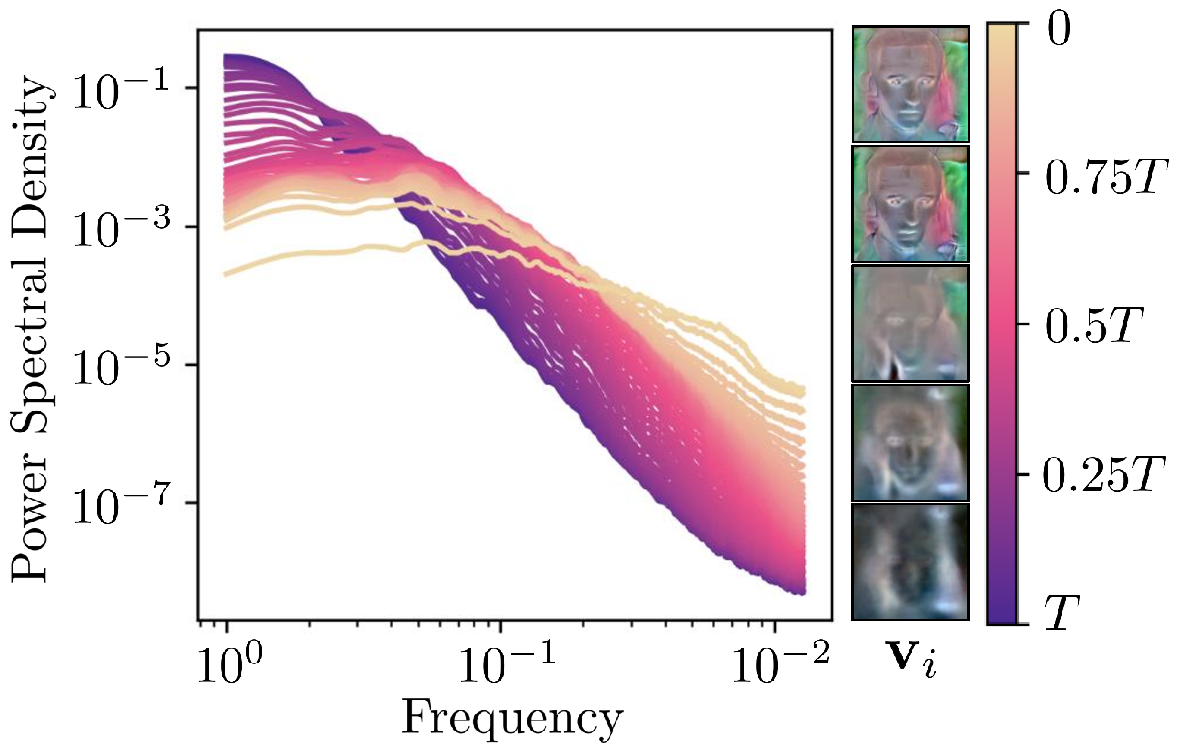
\includegraphics[width=6cm]{figure/PSD.pdf}
    \vspace{-1.5em}
    \caption{\textbf{{Power Spectral Density (PSD) of latent basis.}} {The PSD at $t = T$ (purple) exhibits a greater proportion of low-frequency signals, while the PSD at smaller $t$ (beige) reveals a larger proportion of high-frequency signals. The latent vectors $\vv_i$ are min-max normalized for visual clarity.}
    %\textbf{Power Spectral Density of latent basis}
    %The PSD at $t = T$ (purple line) shows a larger portion of
    %low-frequency signals, whereas the PSD at smaller $t$ (beige line) shows a larger portion of high-frequency signals. The latent vector $\vv_i$ are min-max normalized for visual purposes.
    }\label{figure:PSD}
    \vspace{-2em}
\end{wrapfigure}


In this subsection, we demonstrate how the latent structure evolves during the generative process and identify three trends. 
%\textcircled{\raisebox{-0.9pt}{1}} 
1) {The frequency domain of the latent basis changes from low to high frequency. It agrees with the previous observation that DMs generate samples in coarse-to-fine manner.} % The frequency domain of latent basis changes from coarse to fine feature as the generative process progresses. % (\sref{sec:evolution-x})
%\textcircled{\raisebox{-0.9pt}{2}} 
2) The difference between the tangent spaces of different samples increases over the generative process. It implies finding generally applicable editing direction in latent space becomes harder in later timesteps.
 % and show the possibility of parallel transport on a local basis. (\sref{sec:evolution-samples})
%\textcircled{\raisebox{-0.9pt}{3}} 
3) The differences of tangent spaces {between} timesteps depend on the complexity of the dataset.

% We examine the frequency domain of the local latent basis from different timesteps using the power spectral density (PSD), and find that DMs become more attuned to finer features as the process progresses. 
% We also investigate variations in the local tangent space using the geodesic metric, showing that simpler data leads to greater similarity in the local tangent subspace at different timesteps. This suggests that simpler data leads to increasingly similar features processed at each timestep.
% 이 관찰으로부터 서로 다른 timestep 유사한 signal 을 처리하지 않도록 timestep 을 배치하니 uniform timestep 에 비해 더 좋은 sampling fidelity 를 얻을 수 있었다. 




\paragraph{{Latent bases gradually evolve from low- to high-frequency structures.}}
%\paragraph{latent basis evolves from low frequencies to high frequencies.}
% \paragraph{The frequency domain of latent basis evolves from low-to-high.}
\label{sec:evolution-x}



% In \sref{sec:local}, we observed that coarse manipulations are performed at the beginning of the denoising step, and then finer manipulations are performed as the timestep progresses. 
% To quantitatively verify this observation, we plotted the power spectral density (PSD) of the discovered latent basis. 

\fref{figure:PSD} is the power spectral density (PSD) of the discovered {latent} basis over various timesteps. 
The early timesteps contain a larger portion of low frequency than the later timesteps and the later timesteps contain a larger portion of high frequency.

This suggests that the model focuses on low-frequency signals at the beginning of the generative process and then shifts its {focus} to high-frequency signals over time.
This result strengthens the common understanding
about the coarse-to-fine behavior of DMs over the generative process \cite{choi2022perception, daras2022multiresolution}.



% \yh{This result strengthens the common understanding that DMs start to create coarse features and gradually refine them over a generative process.}
% This suggests that the model focuses on low-frequency signals at the beginning of the generative process and then shifts its attention to high-frequency signals over time.
% long version
% \yh{
% In the forward diffusion process, high-frequency details are perturbed faster than low-frequency signals. Therefore, as the diffusion timestep approaches $t \approx T$, only the low-frequency signals remain in the image. Hence, it is reasonable for a model to reconstruct the original image by focusing on the remaining low-frequency signals.
% }
% short version
% \yh{
% Considering high-frequency perturbed faster in forward diffusion process, it is natural for model to focus on low-frequency signal when $t \approx T$.
% }
% The PSD plots for additional datasets are provided in \aref{appendix:PSD}. Note that each dataset demonstrates a consistent qualitative trend.

% \begin{wrapfigure}{R}{5cm}
% \vspace{-2em}
% 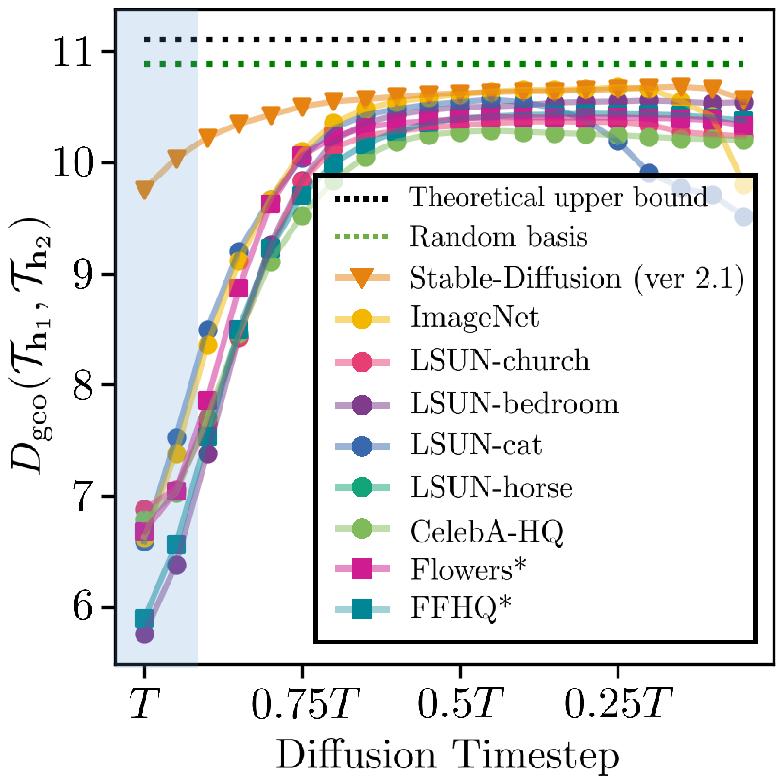
\includegraphics[width=5cm]{figure/Homogenity_samples.pdf}
% \vspace{-2em}
% \caption{
% \textbf{Geodesic distance across tangent space of different samples in various diffusion timesteps}
% Each point represents the average geodesic distance between pairs of 15 samples. 
% The tangent spaces of different samples are only similar early in the generative process.
% }
% \label{homogenity-sample}
% % \vspace{-2em}
% \label{fig:homo}
% \end{wrapfigure}



\paragraph{{The discrepancy of tangent spaces from different samples increases along the generative process.}}
%\paragraph{The difference between the tangent spaces from various samples increases as the generative process progress.}
\label{sec:evolution-samples}

% In our previous findings, we investigated the evolution of the latent basis. The next step is to focus on the evolution of the basis's corresponding {\it ``representation''}, i.e. tangent space. % original 아래
% From now on, we are going to turn our attention to the evolution of the  corresponding {\it ``representation''}, i.e. tangent space.



% In our previous findings, we established that the signal frequency in DM undergoes changes depending on the timestep. In order to gain further insights, we will now examine the representation of the local basis. 

% It is important to emphasize that the local basis is extracted from each local tangent space. This allows us to utilize the geodesic metric to assess the similarity between the discovered local subspaces across various samples, considering the local tangent subspaces generated at different timesteps.
%As a starting point, we checked how similar the discovered local subspaces of the different samples are to each other. 
% To begin, we examined the similarity between the discovered local subspaces across different samples.
% As a starting point, we checked how similar the local tangent spaces $\mathcal{T}_{\mathbf{h}}$ of the different samples are to each other. 
% The distortion of different vector spaces can be measured by the Grassman metric. 

% \begin{wrapfigure}{r}{3.2cm}
% % \vspace{-3em}
% 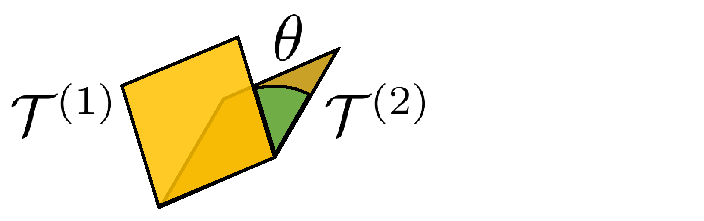
\includegraphics[width=3.2cm]{figure/geodesic_metric.pdf}
% \vspace{-1em}
% \caption{Conceptual illustration of geodesic metric}\label{fig:geodesic_metric}
% \vspace{-1.25em}
% \label{fig:homo}
% \end{wrapfigure}


To investigate the geometry of the tangent basis, we employ a metric on the Grassmannian manifold. The Grassmannian manifold is a manifold where each point is a vector space, and the metric defined above represents the distortion across various vector spaces.
% By employing a metric on the Grassmannian manifold, one can determine the extent of distortion across various vector spaces.
We use \emph{geodesic metric}~\cite{choi2021not, ye2016schubert} to define the discrepancy between two subspaces $\{\mathcal{T}^{(1)}, \mathcal{T}^{(2)}\}$: 

% The distortion of different vector spaces can be found by the Grassman metric. We use \emph{geodesic metric}~\cite{choi2021not, ye2016schubert} to define the distortion between two local latent subspace centered at $\{\vh^{(1)}, \vh^{(2)}\}$: 

% \begin{figure}[h]
%    \centering
%    \vspace{-10pt}
%    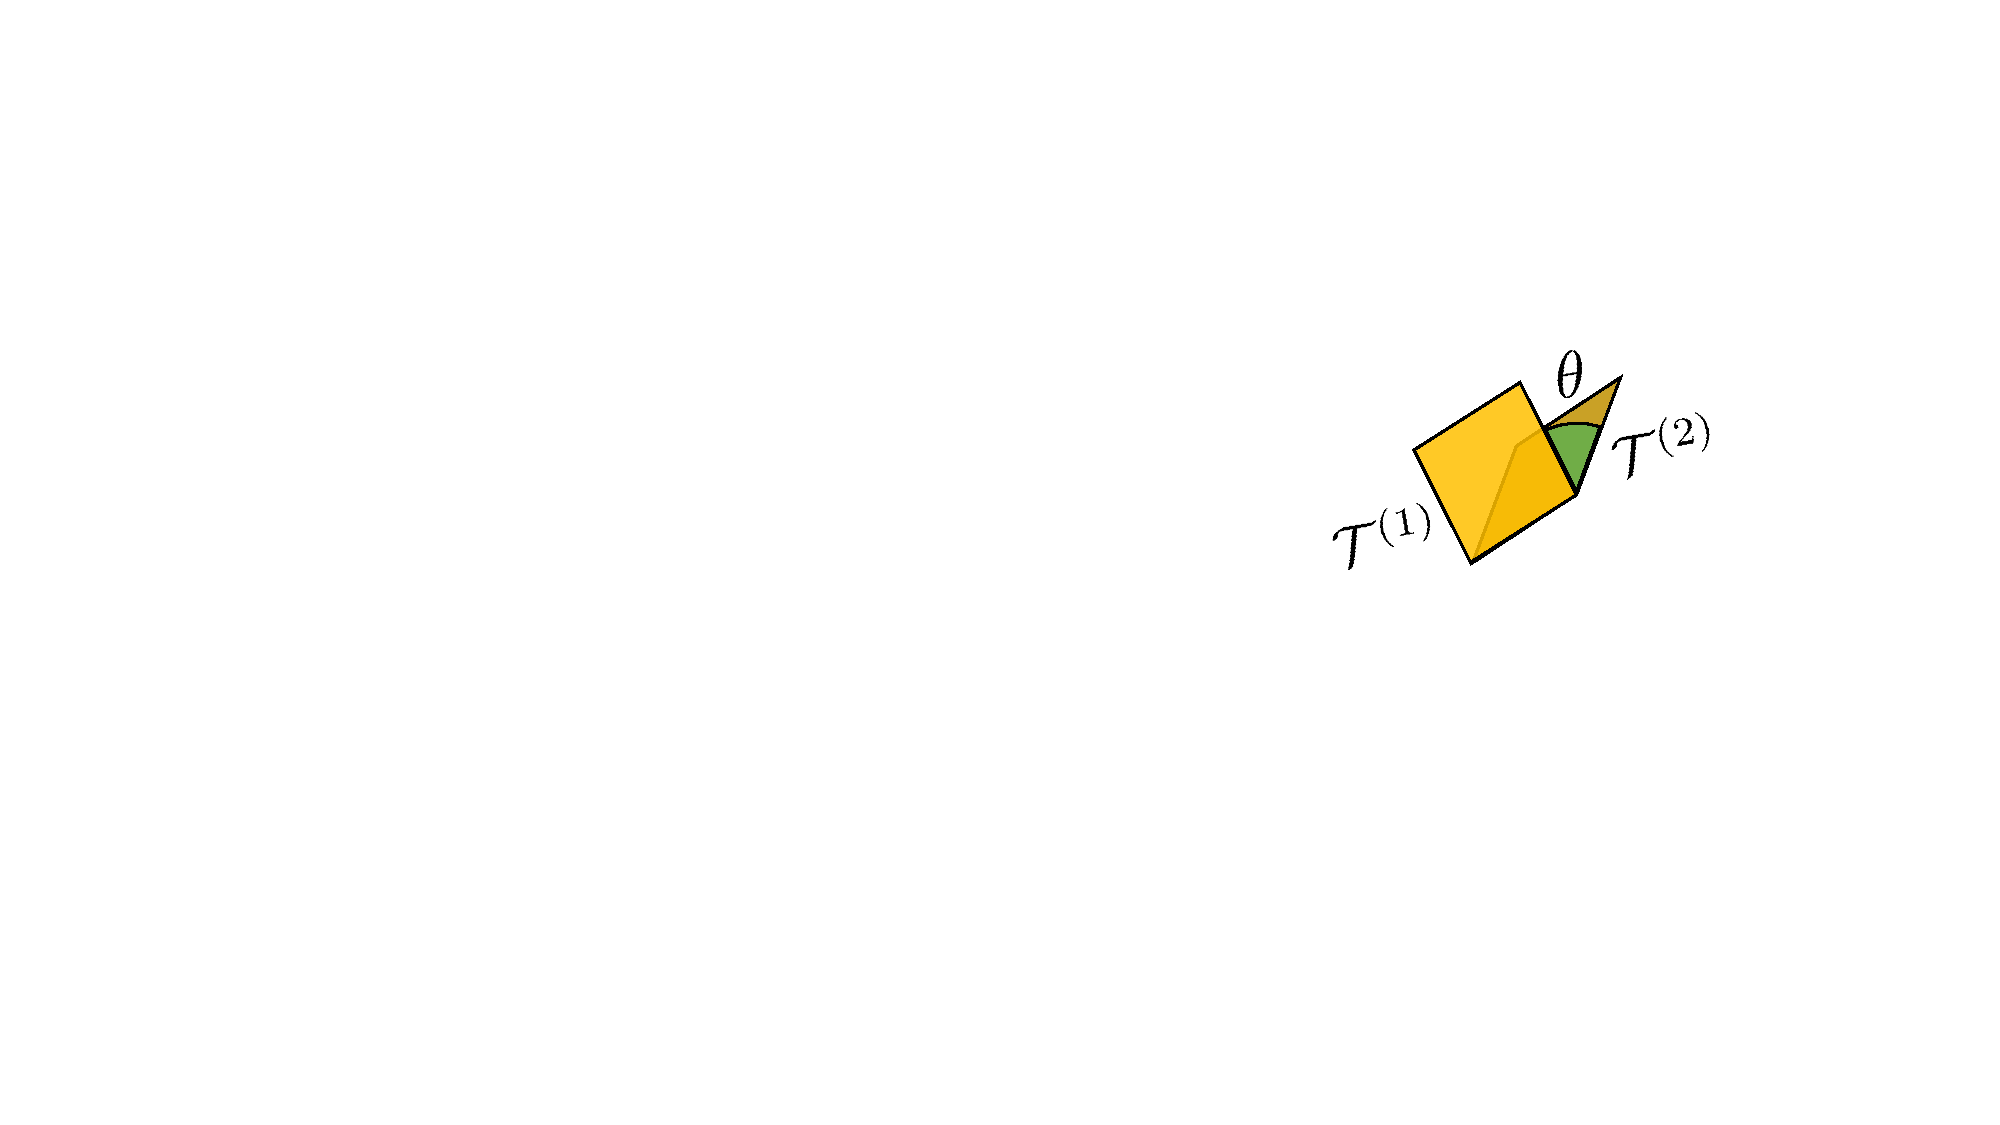
\includegraphics[height=40pt,right]{figure/geodesic_distance_mini.pdf}
%    % \vspace{-10pt}
%    \vspace{-60pt}%
%    \label{fig:cclogo}
% \end{figure}

%%% Small Geodesic metric figure
% \begin{figure}[h]
%    \centering
%    \vspace{-10pt}
%    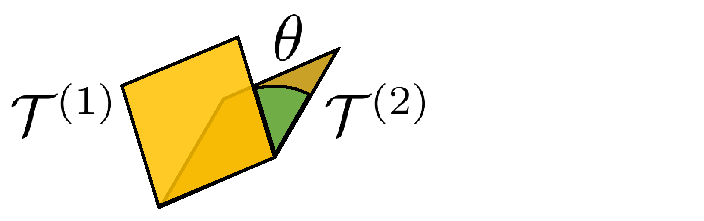
\includegraphics[height=30pt,right]{figure/geodesic_metric.pdf}
%    % \vspace{-10pt}
%    \vspace{-60pt}%
%    \label{fig:cclogo}
% \end{figure}

\begin{equation}
D_{\text{geo}}(\mathcal{T}^{(1)}, \mathcal{T}^{(2)}) = \sqrt{\sum_k \theta_k^2},
\end{equation}


\begin{wrapfigure}{r}{6cm}
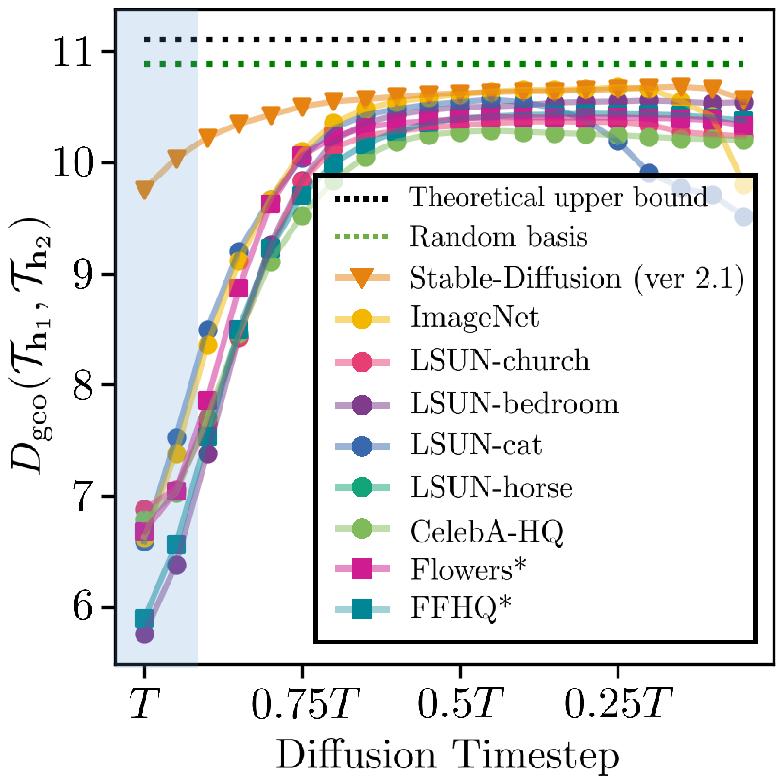
\includegraphics[width=5cm, center]{figure/Homogenity_samples.pdf}
    \vspace{-1em}
    \caption{
    \textbf{Geodesic distance across tangent space of different samples {at} various diffusion timesteps.}
    Each point represents the average geodesic distance between pairs of 15 samples.
    { It is notable that the similarity of tangent spaces among different samples diminishes as the generative process progresses.}
    %The tangent spaces of different samples are only similar early in the generative process.
    }
    \label{homogenity-sample}
\vspace{-3em}
\label{fig:homo}
\end{wrapfigure}


\begin{figure}[!b]
    \centering
    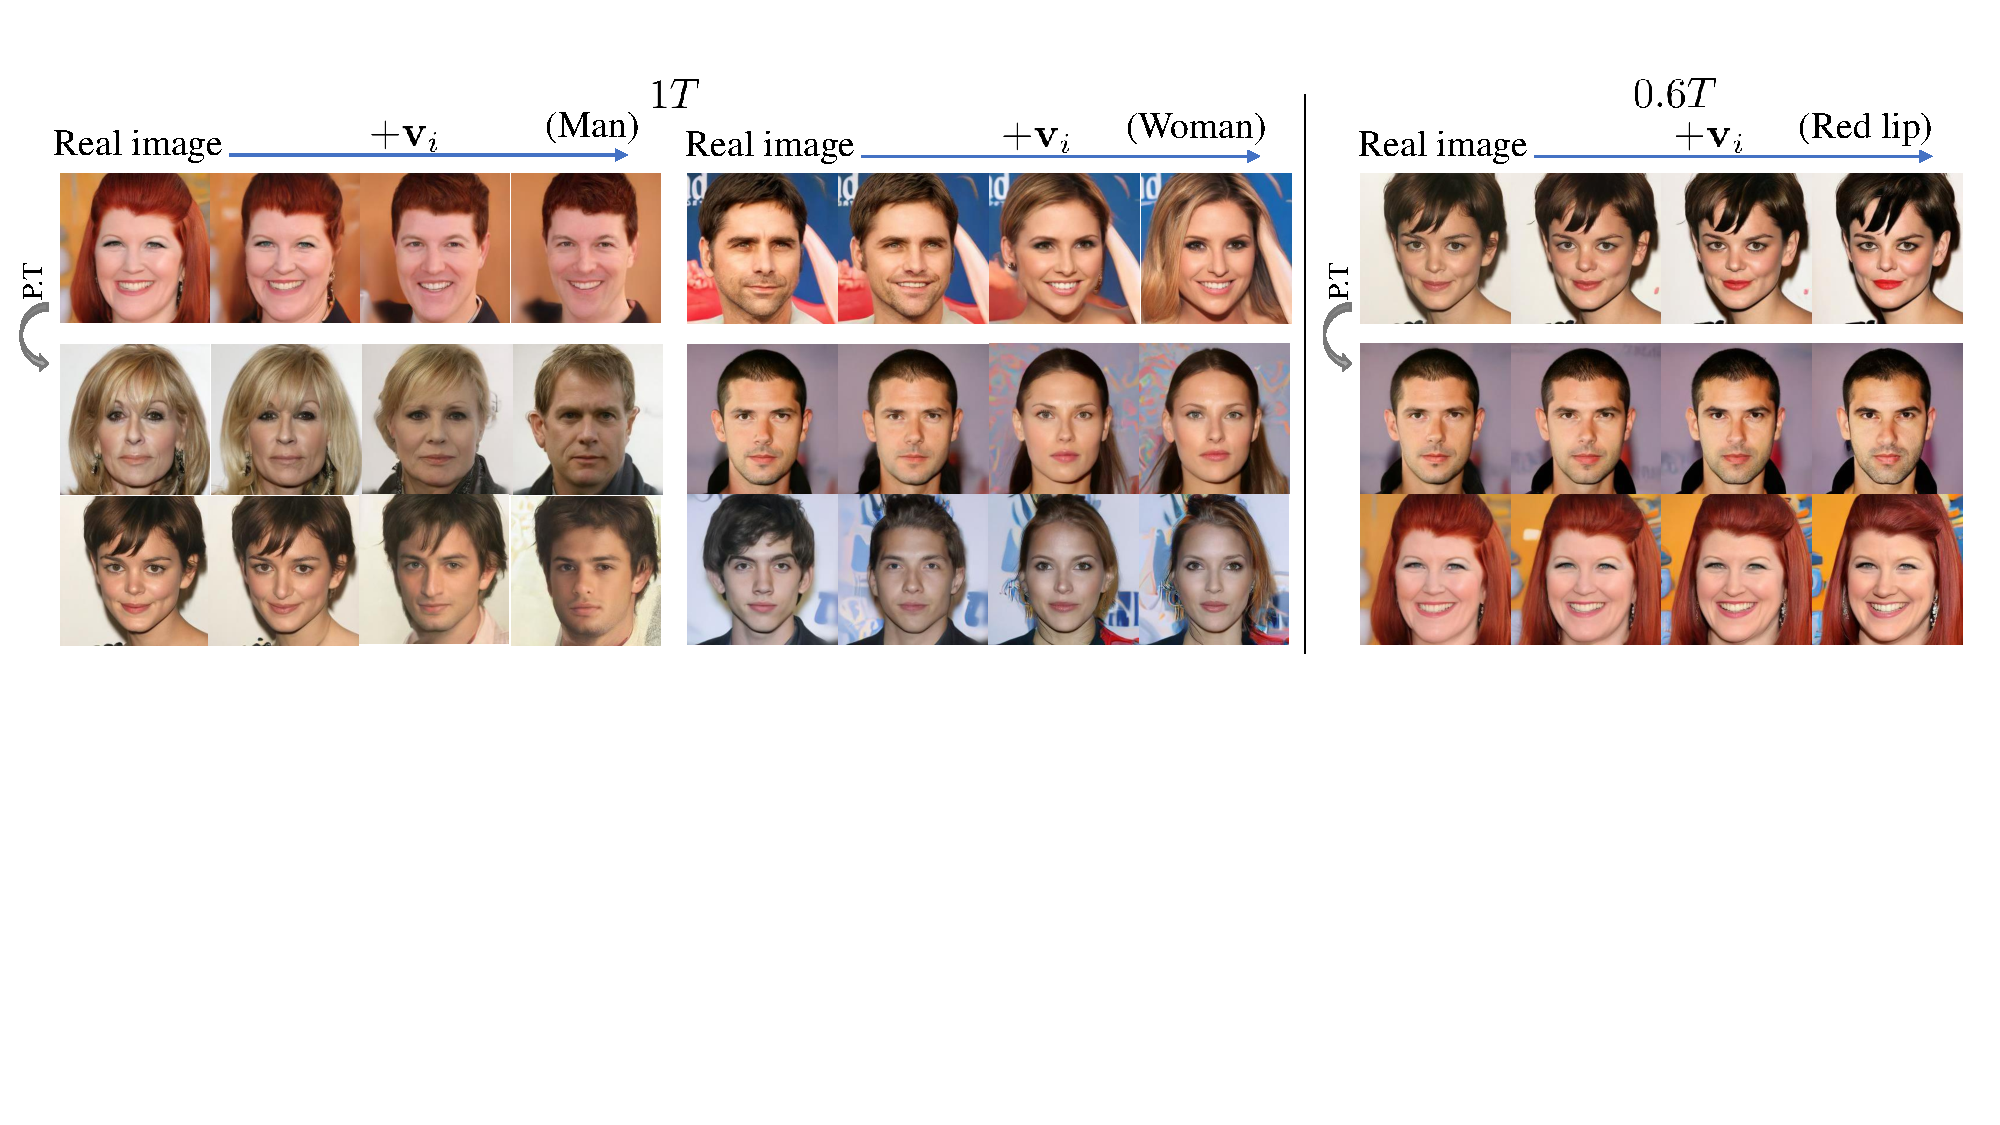
\includegraphics[width=1\linewidth]
    {figure/parallel_tmp.pdf}
    % \vspace{-1em}
    \caption{\textbf{\jo{Examples of image edition using parallel transport.}}
    \jo{The first row demonstrates the results of editing with their respective latent vectors, while the subsequent rows exhibit the results of editing through the parallel transport (P.T) of the latent vectors used in the first row. The latent vector performs effectively when $t = T$ (left and middle), but comparatively less satisfactorily for $0.6T$ (right).}
    %The first row show the result of editing with their own latent vector, and the rest of the rows show the result of editing with a parallel transport of the first row. The latent vector works well for when $t=T$ (left, middle), but relatively poorly for $0.6T$ (right). 
    }
    % \vspace{-1em}
    \label{fig:parallel}
\end{figure}



where {$\theta_k$} denotes the $k$-th principle angle between $\mathcal{T}^{(1)}$ and $\mathcal{T}^{(2)}$. Intuitively, the concept of geodesic metric can be understood as an angle between two vector spaces.
%(\ifref{fig:geodesic_metric})
{Here, the comparison between two different spaces was conducted for 
$\{\mathcal{T}_{\vh_1}, \mathcal{T}_{\vh_2} \}$. 
Unlike the \exspace{}, the \ehspace{} assumes a Euclidean space which makes the computation of geodesic metric that requires an inner product between tangent spaces easier. 
The relationship between tangent space and latent subspace is covered in more detail in \aref{appendixsec:relationship_tangent_latent}.
}


% \begin{wrapfigure}{r}{6cm}
%     \vspace{-1em}
% 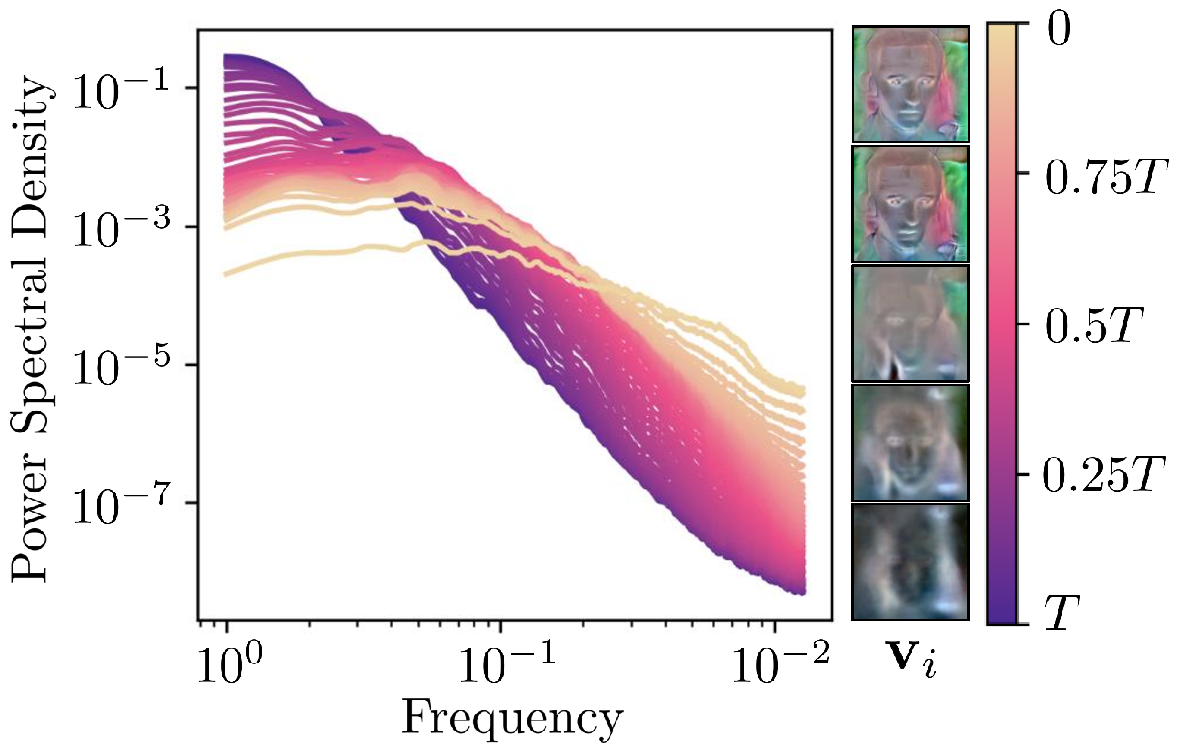
\includegraphics[width=6cm]{figure/PSD.pdf}
%     \vspace{-1.5em}
%     \caption{\textbf{{Power Spectral Density (PSD) of latent basis.}} {The PSD at $t = T$ (purple) exhibits a greater proportion of low-frequency signals, while the PSD at smaller $t$ (beige) reveals a larger proportion of high-frequency signals. The latent vectors $\vv_i$ are min-max normalized for visual clarity.}
%     %\textbf{Power Spectral Density of latent basis}
%     %The PSD at $t = T$ (purple line) shows a larger portion of
%     %low-frequency signals, whereas the PSD at smaller $t$ (beige line) shows a larger portion of high-frequency signals. The latent vector $\vv_i$ are min-max normalized for visual purposes.
%     }\label{figure:PSD}
%     \vspace{+2em}
% \end{wrapfigure}



\fref{fig:homo} demonstrates that the tangent space\uh{s} of the different samples are the most similar at $t=T$ and diverge as {timestep becomes} zero. 
% This aligns with the existing understanding that, after a certain timestep, the reverse diffusion trajectories of different samples are isolated from each other\cite{zhang2022gddim, wu2022uncovering}.


Moreover, the similarity across tangent space{s} allows us to effectively transfer the latent basis from one {sample} to another through parallel transport as shown in \fref{fig:parallel}.
% as showcased in \sref{sec:parallel}. 
% \fref{fig:parallel} demonstrates the edited results of parallel transporting the latent basis obtained from one sample to another sample.
% In $T$, where homogenity of tangent space exists, 
In $T$, {where the tangent spaces are homogeneous},
we consistently obtain semantically aligned editing results. 
{On the other hand, parallel transport at $t=0.6T$ does not lead to satisfactory editing because the tangent spaces are hardly homogeneous. Thus, we should examine the similarity of local subspaces to ensure consistent editing across samples.}
% However, when attempting parallel transport at $t=0.6T$, where homogeneity is lacking, it fails to produce satisfactory outcomes.
% This underscores the significance of considering the similarity of local subspaces.



% This is corroborated by the results depicted in \fref{fig:parallel}. 
% By transferring the local semantic direction from the first sample to subsequent samples, we consistently obtain semantically aligned editing results. However, it is important to note that when attempting to transfer the local basis at $t=0.6T$, where homogeneity is lacking, the parallel transport method fails to produce satisfactory outcomes. This underscores the significance of considering the similarity of local subspaces.

% \paragraph{\jo{Simpler datasets exhibit more consistent tangent spaces over timesteps.}}
\paragraph{DMs trained on simpler datasets exhibit more consistent tangent spaces over time.} 
% \paragraph{DMs trained on simple datasets have similar tangent spaces across different timesteps.} 
% \paragraph{Tangent basis evolves less if trained on simple dataset}
\label{sec:evolution-t}
% \modify{frequency는 다른데, 과연 그 representation도 많이 다를까? -> tangent space에서의 유사함은 representation의 유사함을 말한다. 이런 직관 설명 내용 추가.}
% In the previous section, we studied the evolution of the tangent space by comparing it across different samples. This time, we compare tangent space across different timesteps.
% In the previous section, we studied the evolution of the tangent space by comparing different samples. This time, we investigate how the tangent space change by comparing it across different timesteps.

% This suggests that the local latent basis that the model pays attention to at each point in time is similar. To help readers understand this, we illustrate in Figure 1b how much of the original feature captured by vector vi is lost when we transport it from one timestep to another, using parallel transport from t = T to 0.1T. As expected, when the local tangent space is similar, the transported vector maintains its existing signal, but it loses this pattern as we move further away from the original timestep. We found this relationship between local tangent space and local semantic subspace to hold true for all datasets. For a more detailed discussion, please refer to the appendix.

In \fref{fig:timestep} (a), we provide a distance matrix of the tangent spaces across different timesteps, measured by the geodesic metric. 
We observe that the tangent spaces are more similar to each other when a model is trained on CelebA-HQ, compared to ImageNet.
\uh{To verify this trend, we measure the geodesic distances between tangent spaces of different timesteps and plot the average distances of the same difference in timestep in \fref{fig:timestep} (b)}.
% To verify this trend, in \fref{fig:timestep} (c), we measured the average geodesic distance of the tangent space according to the difference of diffusion timesteps.
As expected, we find that DMs trained on datasets, that are generally considered simpler, have similar local tangent spaces over time.

% 눈으로 봤을때, 우리는 CelebA-HQ 와 같이 비교적 단순한 dataset 에 대해 학습한 경우, ImageNet 과 같이 복잡한 dataset 을 학습했을때와 비교했을때 시간 별 local tangent space 가 유사한 것을 확인할 수 있었다.
% In \fref{fig:timestep} (c), 이를 검증하기 위해 우리는 여러 dataset 에서 학습한 DM 의 timestep 거리별 local tangent space 의 평균 거리를 측정했다. 
% 기대한대로, 일반적으로 더 단순하다고 여겨지는 데이터셋에 학습한 DM 일수록 (e.g. CelebA-HQ > LSUN > ImageNet) 시간별 local tangent space 가 유사함을 확인할 수 있었다. 


% 
% parallel transport 부분은 appendix 로 넘기기
% 
% Notice that the similarity between tangent spaces implies \uh{consistency of latent basis across timesteps}. %a consistent latent basis at each timestep.
% In \fref{fig:timestep} (b), we parallel transport the latent vector $\vv_i$ to various tangent spaces and visualize the outcomes.
% As expected, when the tangent spaces are similar, the transported vector ${\vv'}_i$ retains the original signal. On the other hand, as we move to more distant timesteps, where the tangent space is farther apart, ${\vv'}_i$ deviates from the original signal.

% When the tangent space is similar, the transported vector ${\vv'}_i$ retains the original signal. However, when moved to a distant regime, ${\vv'}_i$ deviates from the original signal.
% The relationship between tangent space and latent subspace is covered in more detail in \aref{appendixsec:relationship_tangent_latent}.

% mingi
% In \fref{fig:timestep} (b), 이렇게 local tangent space 간 거리가 작은 경우, 우리는 
% In \fref{fig:timestep} (b), the similarity of local tangent space is indirectly visualized through the local basis $v_1$. \modify{b는 tangent space에서의 변화가 semantic subspace에서는 어떤지 보여주는 것이라는 설명 추가.} To aid visualization, we perform parallel transport of the local basis at T and 0.1T to the local tangent space at different time steps. These visualizations also confirm the similarity of tangent spaces between time steps. \modify{이러한 경향성은 모든 샘플들에 대해 나타나며, 이는 appendix봐라 라고 말하고, 이전에 넣어두었던 피규어 appendix에 넣기.}

% mingi
% Furthermore, we have observed a correlation between the difference in tangent space at various time steps and the complexity of the dataset. \fref{fig:timestep} (c) illustrates the average geodesic distance of the tangent space according to the disparity in time steps.  \modify{서로 다른 타임스텝에서 얼마나 급격하게 변화하는지 보여주고 있따~~ 추가} Both \fref{fig:timestep} (a) and (c) demonstrate that in the case of ImageNet, which is considered a highly complex dataset, the tangent spaces across time steps exhibit less similarity compared to CelebA-HQ, which is deemed a less complex dataset.

% Simple dataset 에서는 timestep 별 semantic structure 의 homogenity 를 만들어낸다.
% The simpler the data, the more similar the Local Tangent Basis per timestep.

% \begin{figure}[!t]
%     \centering
%     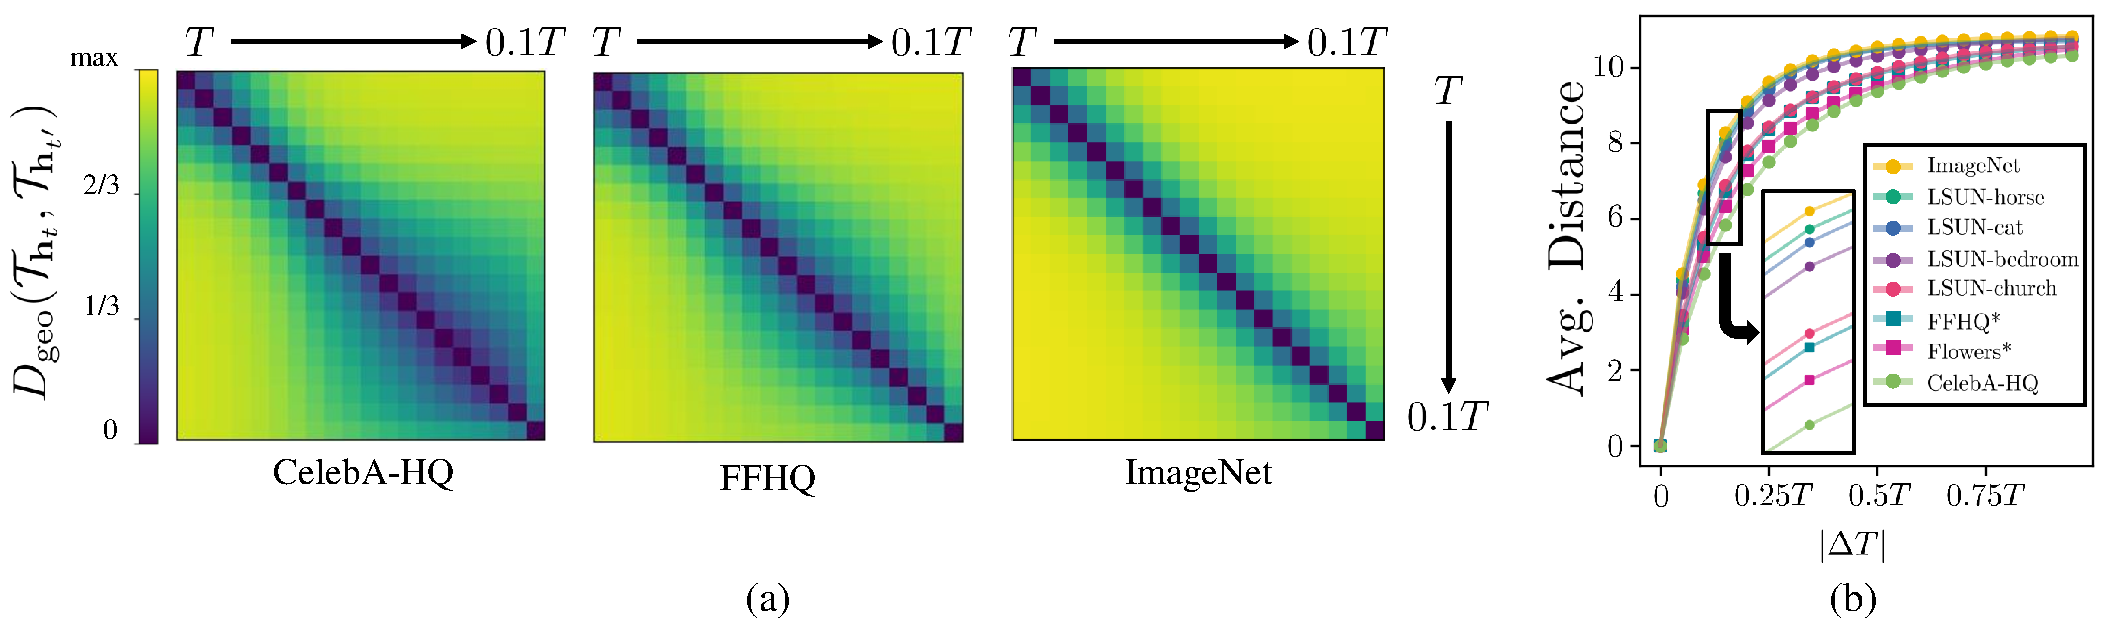
\includegraphics[width=0.9\linewidth]{figure/evolution-t-no_pt.pdf}
%     \caption{
%     \textbf{Models trained on simple datasets have similar tangent spaces at different timesteps.}
%     (a) Visualization of the distance matrix of tangent space across various timesteps measured by geodesic metric. 
%     (b) Average geodesic distance according to the difference of diffusion timestep.
%     It shows that the average distance is closer in CelebA-HQ compared to LSUN, and LSUN compared to ImageNet.
%     }
%     \label{fig:timestep}
% \end{figure}


\begin{figure}[!t]
    \centering
    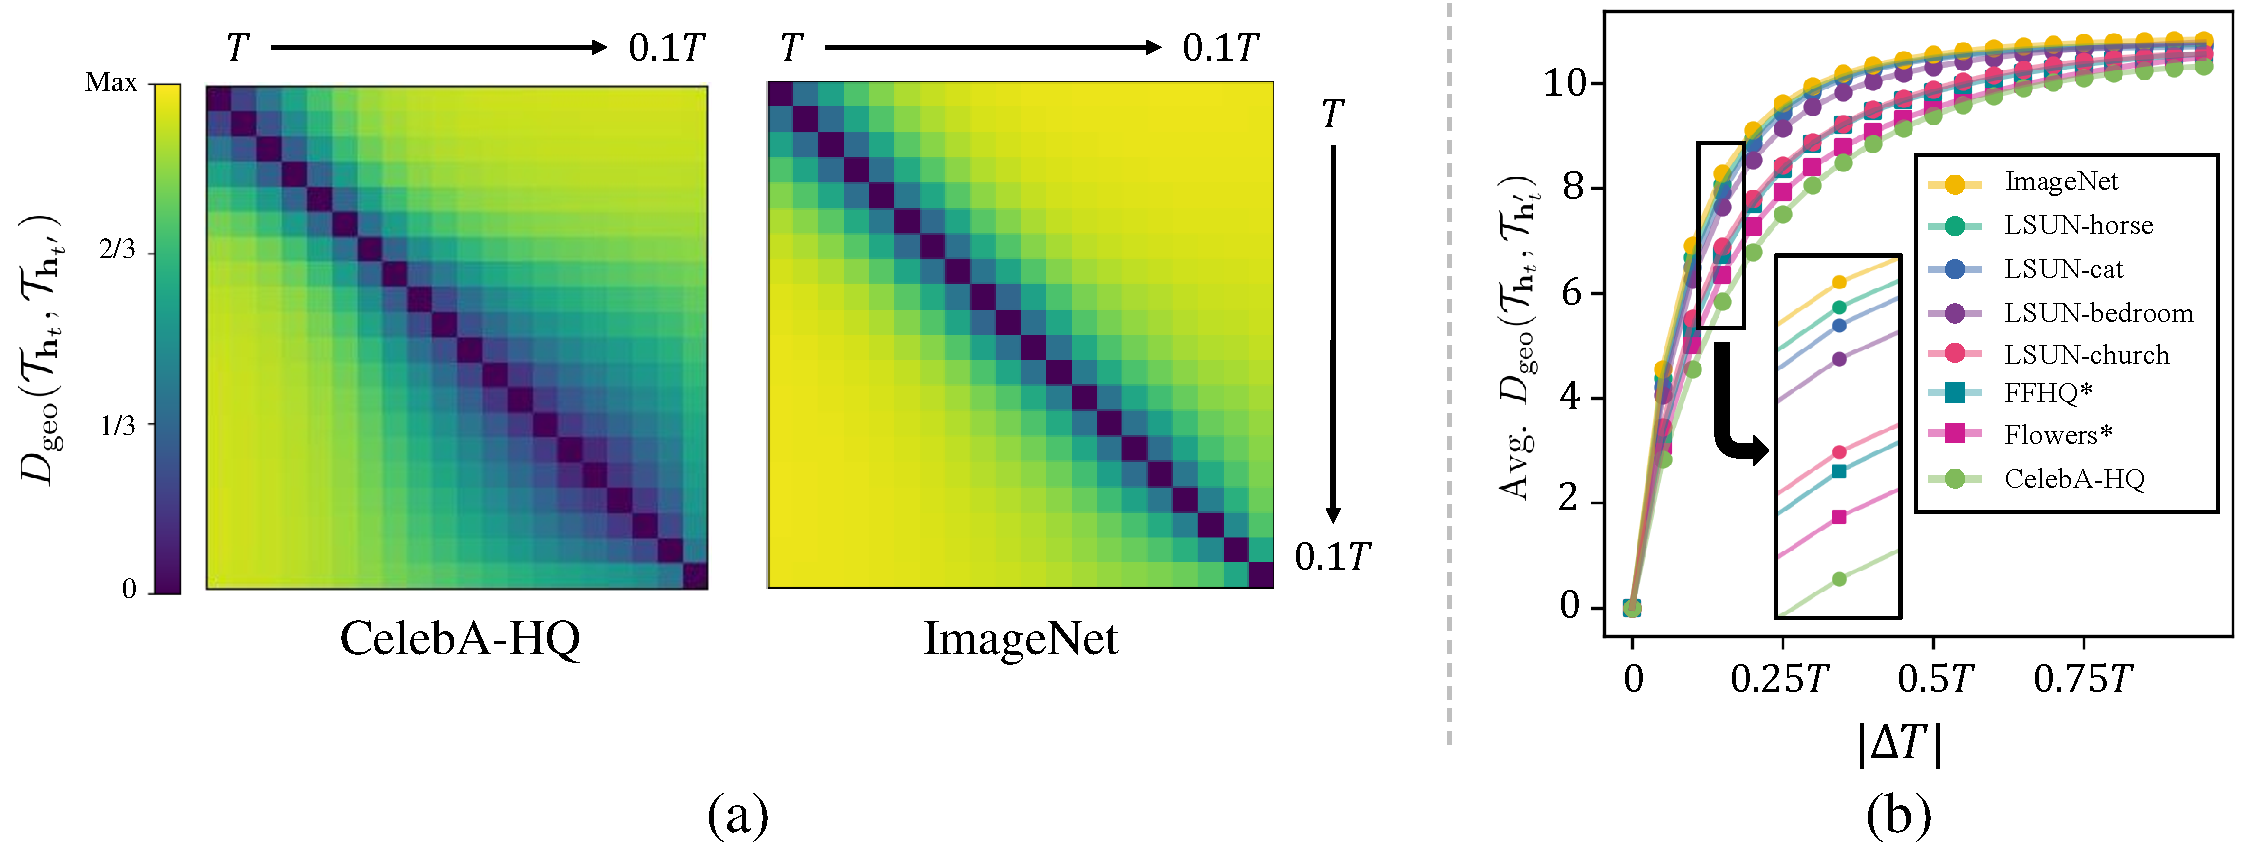
\includegraphics[width=0.9\linewidth]{figure/evolution-t-simple.pdf}
    % 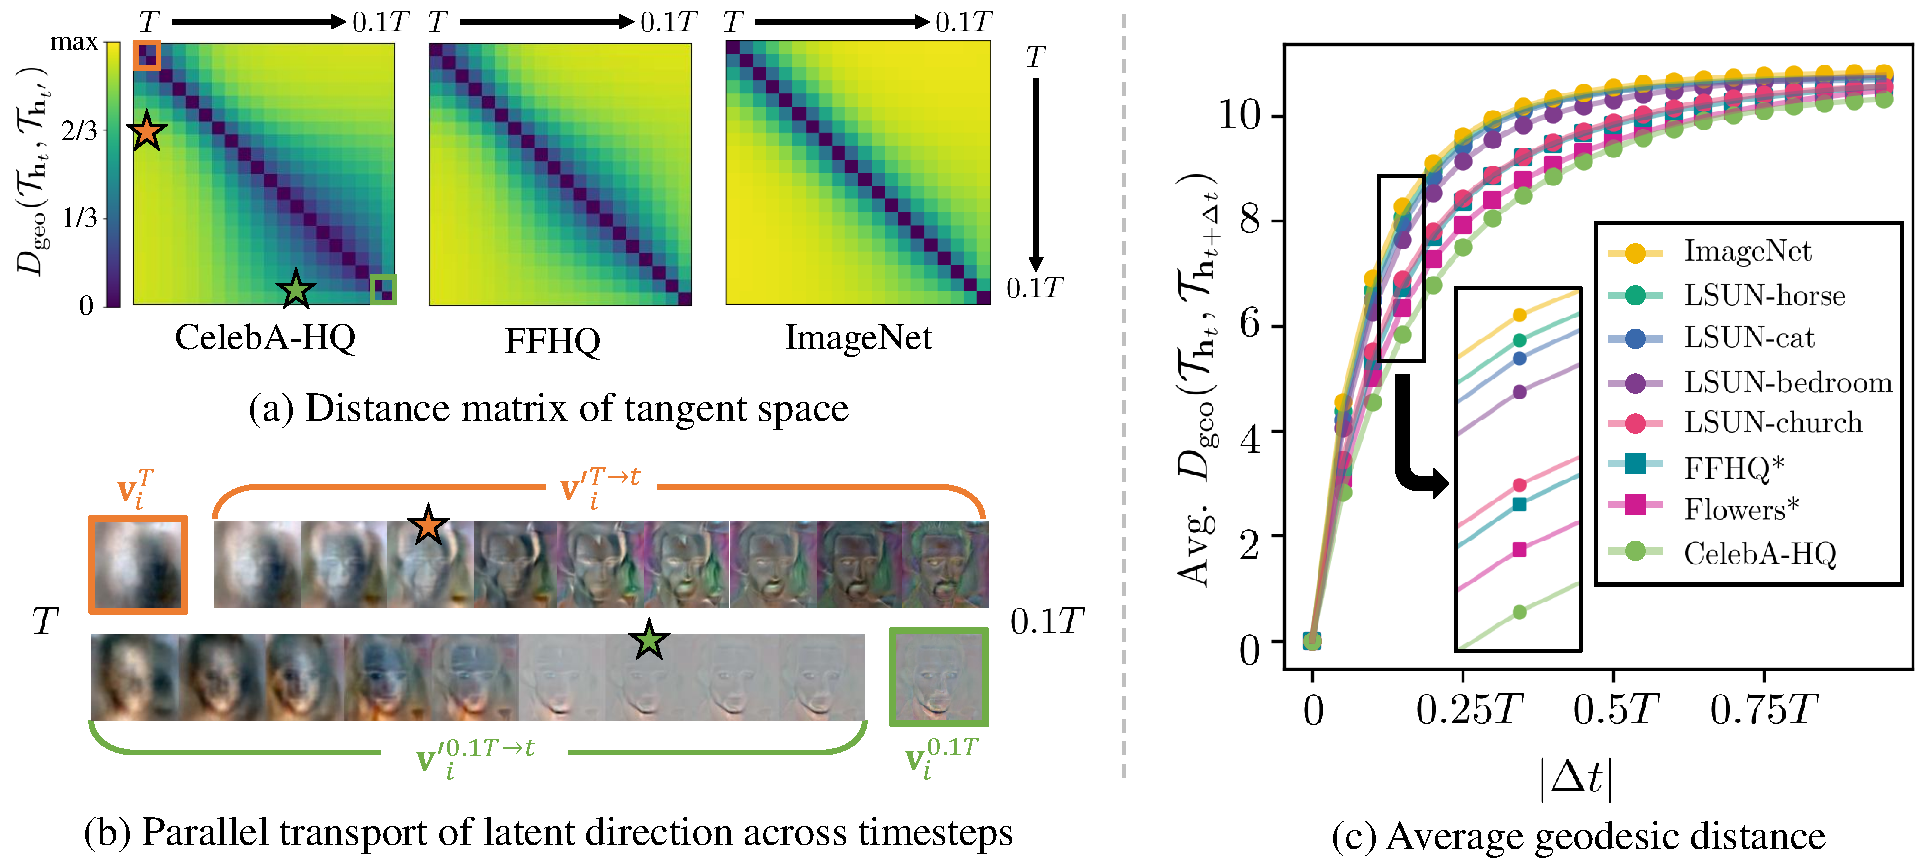
\includegraphics[width=0.9\linewidth]{figure/evolution-t.pdf}
    \vspace{-0.5em}
    \caption{
    \textbf{\jo{Simpler} datasets lead to \jo{more} similar tangent spaces across diffusion timesteps.}
    % \textbf{Models trained on simple datasets have similar tangent spaces at different timesteps.}
    \jo{(a) Distance matrix visualization of tangent space measured by geodesic metric across various timesteps.}
    %(a) Visualization of the distance matrix of tangent space across various timesteps measured by geodesic metric. 
    % (b) Visualization of the result from parallel transport across timesteps. \yh{${\vv'}_i^{t_a \rightarrow t_b}$ denotes the latent vector transported from $t_a$ to $t_b$. Transported vector significantly deviates from the original vector, as the tangent space grows further apart according to the distance matrix. For visualization purposes, $\vv_i$ \jo{is min-max normalized}.} %undergoes min-max normalization.}
    (b) Average geodesic distance \jo{based on timestep differences, indicating that the complexity of the dataset correlates with greater distances between tangent spaces.}
    %according to the difference of  timestep. It shows that the more complex the dataset, the greater the distance between tangent spaces.
    }
    \vspace{-1em}
    \label{fig:timestep}
\end{figure}

% 앞에서 우리는 DM 이 민감하게 반응하는 signal 의 frequency 가 timestep 에 따라 변화함을 확인했다. 그렇다면, 그 representation 은 어떨까?
% 이를 확인하기 위해, 이미지를 생성해나가는 과정의 각 timestep 에서 만들어지는 local tangent subspace 간 geodesic metric 을 측정했다. 

%%% ICML ver
% We further investigate the coarse-to-fine editing along the generative process from timestep $T$ to $0$. \fref{fig:PSD} (a) shows the example directions $\vv_i$ across different timesteps. At $T$, $\vv_i$ leads to coarse attribute changes in $\vx_0$ by blurry change in $\vx_T$. At $0.25T$, $\vv_i$ edits high-frequency details in both $\vx_0$ and $\vx_t$. \fref{fig:PSD} (b) shows the power spectral density (PSD) of $\vv_i$. We compute the PSD by taking $\vv_1, ..., \vv_{10}$ from 20 samples. The early timesteps contain a larger portion of low frequency than the later timesteps and the later timesteps contain a larger portion of high frequency. This phenomenon agrees with the tendency in the edited images. This results strengthens the common understanding of the timesteps~\cite{kwon2022diffusion,choi2022perception, daras2022multiresolution}.

\begin{figure}[!t]
    \centering
    \vspace{+1em}
    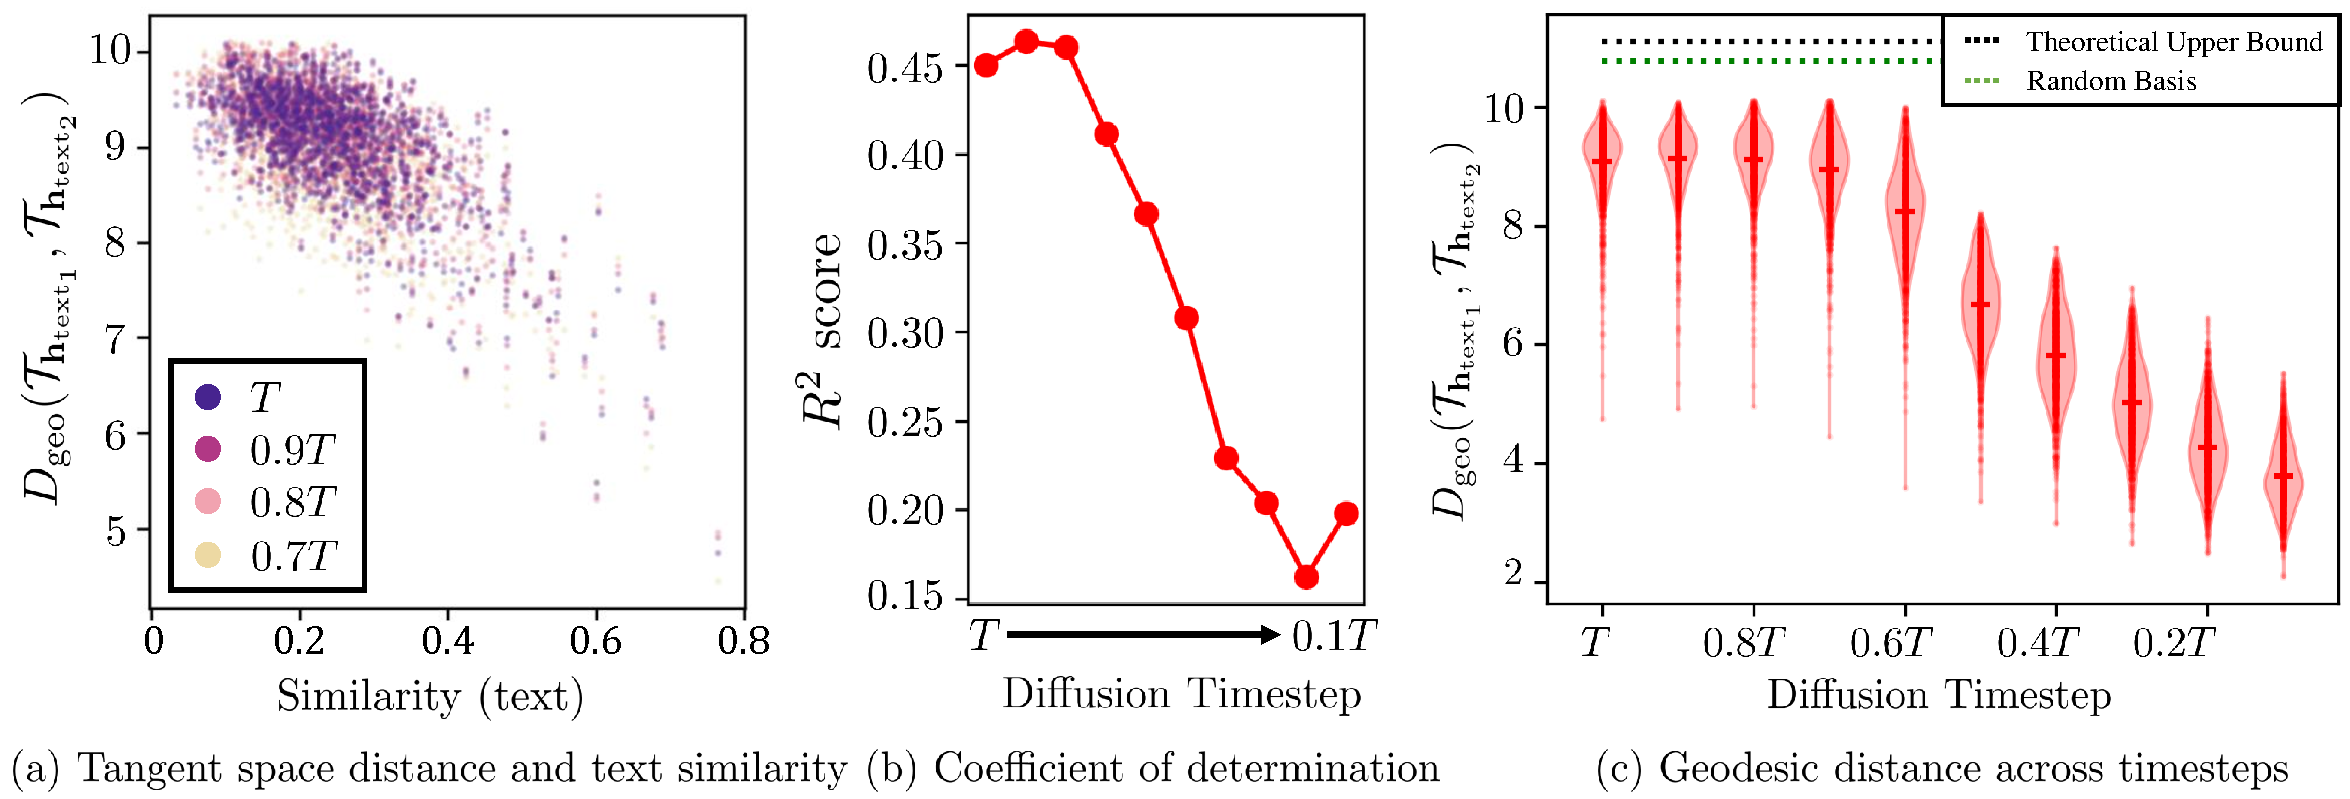
\includegraphics[width=0.9\linewidth]{figure/Homogenity_prompts.pdf}
    % 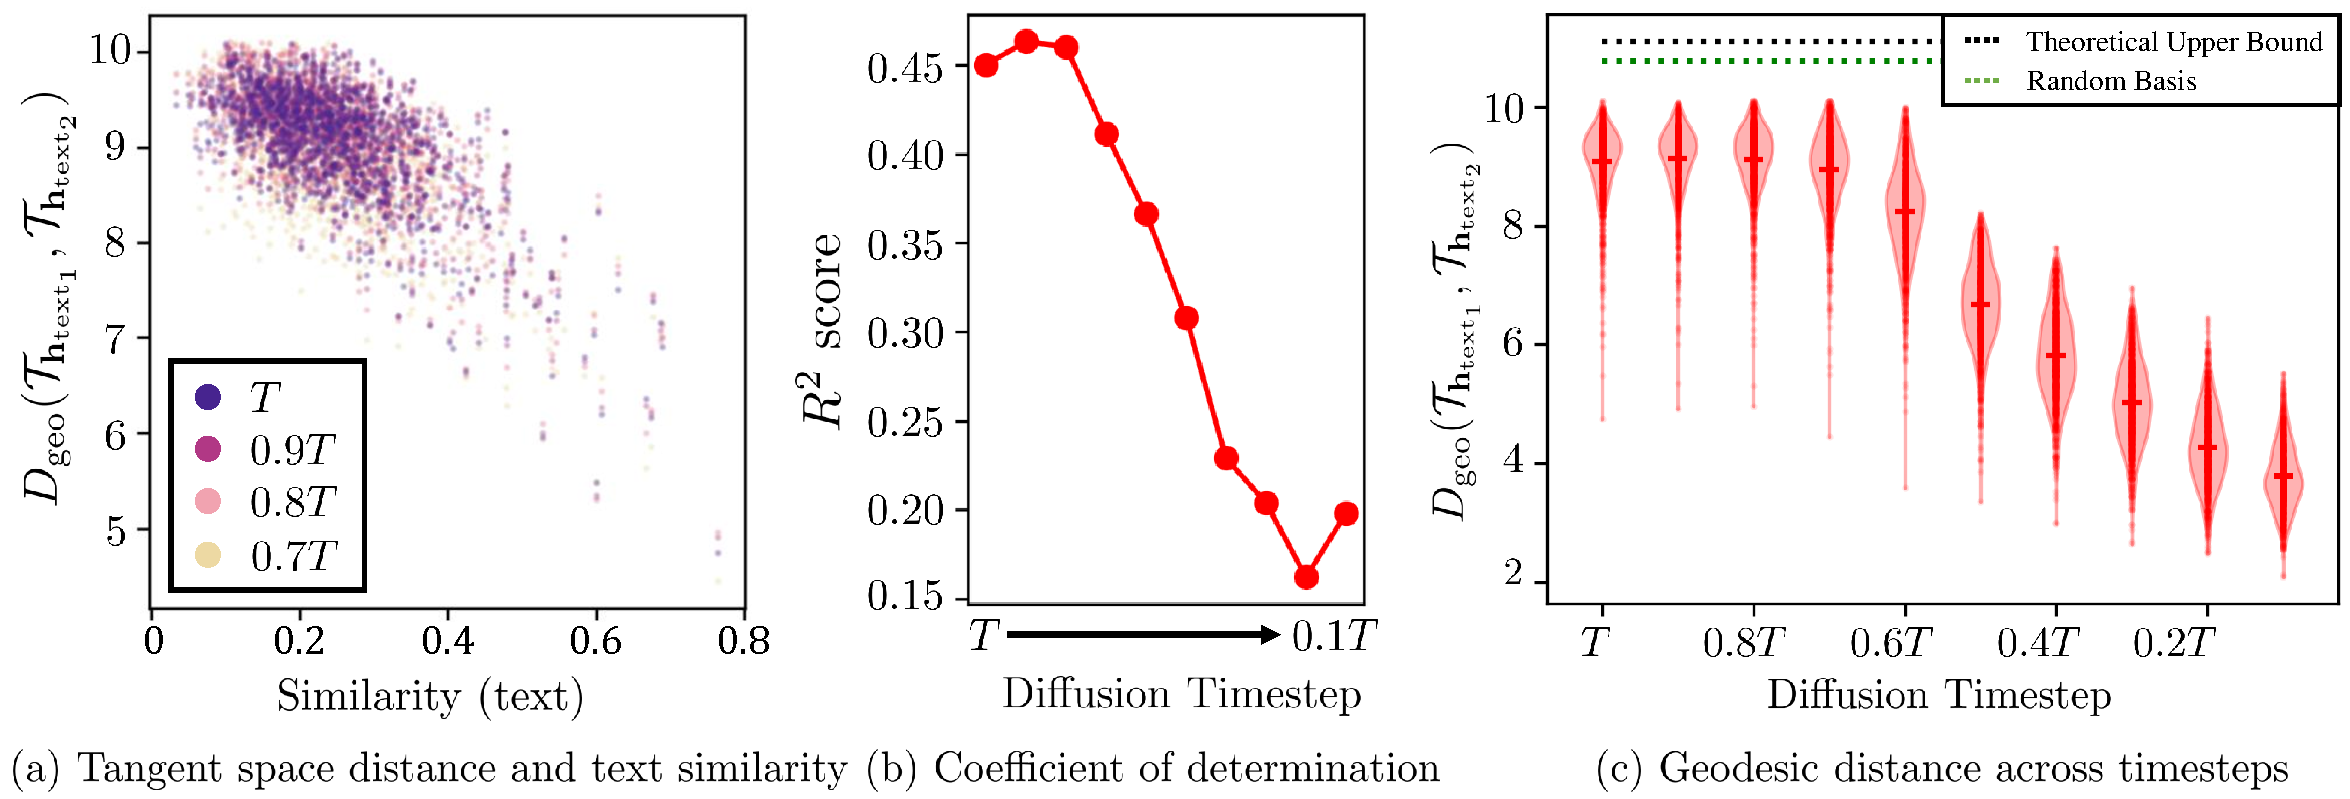
\includegraphics[width=0.9\linewidth]{figure/Homogenity_prompts.pdf}
    % \vspace{-1em}
    \caption{
    \textbf{Similar prompt\jo{s} create similar tangent space\jo{s}, and the \jo{impact of the prompt decreases as the generative process progresses.}} 
    (a) \mingi{The horizontal axis represents the CLIP similarity between two different prompts, \jo{while} the vertical axis represents the geodesic distance in the tangent space from each prompt.} \jo{Different colors represent various diffusion timesteps. A negative relationship is observed between prompt similarity and tangent space distance.}
    %Different diffusion timesteps are denoted as different colors.}
    % \modify{The clip similarity between two different prompts and the geodesic distance in the tangent space created from each respective prompt.}
    % Different colors denote different diffusion timesteps.
    %There is a negative relationship between prompt similarity and tangent space distance.
    %\textbf{The \jo{impact of the prompt as the generative process progresses.}} 
    % \textbf{The influence of the text decreases as the generative process progresses.} 
    (b) The $R^2$ score of the linear regression between clip similarity and geodesic distance of tangent spaces decreases \jo{throughout} the generative process.
    (c) Each point represents the distance between tangent spaces created from different prompts. Until around $t = 0.7T$, the distance between tangent spaces is very large, but it gradually \jo{decreases thereafter.}
    %becomes closer afterward. 
    This indicates that the influence of the prompt on the tangent space diminishes.
    }
    % \vspace{-1em}
    \label{fig:stable_text}
\end{figure}

%\subsection{How the Text-Condition Controls the Geometry of DMs?}
\subsection{\uh{Effect of conditioning prompts on the latent structure}}
% \subsection{\jo{Text-conditioned control of geometry in latent spaces}}
\label{sec:text}
% In this subsection, we aim to find how prompts controls the generative process in geometrical perspective. 
% To demonstrate this, we analyze local semantic subspace and tangent space from randomly sample 50 captions from the MS-coco dataset \cite{lin2014microsoft}. Here we used $\vx{} \sim \mathcal{N}(0, \textbf{I})$ for latent variable.
% To explore this, we randomly sample 50 captions from the MS-coco dataset \cite{lin2014microsoft} and analyse the local semantic subspace and local tangent space extracted for $\vx{} \sim \mathcal{N}(0, \textbf{I})$. 

% 이를 살펴보기 위해, MS-coco dataset \cite{lin2014microsoft} 로부터 50개의 caption 을 random sample 한 뒤, $\vx{} \sim \mathcal{N}(0, \textbf{I})$ 에 대해 추출된 local semantic subspace 와 local tangent space 를 분석했다. 
% 앞에서 말했듯이, local semantic subspace 는 모델이 주목하는 signal 에 대응하고, local tangent space 는 그 signal 들에 대응하는 semantic represenation 에 대응한다. 

In this subsection, we aim to investigate how prompts influence the generative process from a geometrical perspective. 
We randomly sampled 50 captions from the MS-COCO dataset \cite{lin2014microsoft} and used them as text conditions.
% For the latent variable, we utilize $\vx{} \sim \mathcal{N}(0, \textbf{I})$. 
% Our objective is to explore the impact of text-conditioning on the geometry of DMs.



\paragraph{Similar text conditions induce similar tangent spaces.}
% \fref{fig:stable_text} depicts the relationship between text and the tangent space. 
In \fref{fig:stable_text} (a), we observe a negative correlation between the CLIP similarity of texts and the distance between tangent spaces. 
In other words, when provided with similar texts, the tangent spaces are more similar. 
 % model have similar tangent spaces.
% This implies why manipulating the local latent basis vector according to the given text will result in a corresponding edit (\ifref{fig:local_basis_text_vk}, \ifref{fig:local_basis_text})
The linear relationship between the text and the discrepancy of the tangent spaces is particularly strong in the early phase of the generative process as shown by $R^2$ score in \fref{fig:stable_text} (b).
% In \fref{fig:stable_text} (b),
% the $R^2$ score indicates that the linear relationship between the text and local tangent space is particularly strong during the early stages of the generative process. 

% In this subsection, we aim to find how prompts controls the generative process in geometrical perspective. 
% To demonstrate this, we analyze local semantic subspace and tangent space from randomly sample 50 captions from the MS-coco dataset \cite{lin2014microsoft}. Here we used $\vx{} \sim \mathcal{N}(0, \textbf{I})$ for latent variable.
% To explore this, we randomly sample 50 captions from the MS-coco dataset \cite{lin2014microsoft} and analyse the local semantic subspace and local tangent space extracted for $\vx{} \sim \mathcal{N}(0, \textbf{I})$. 

\paragraph{\uh{The generative process depends less on text conditions in later timesteps.}}
% \paragraph{\jo{Text-conditioning effects diminish over generative processes.}}
%\paragraph{The effect of the text becomes weaker, as the generative process progresses.}
\fref{fig:stable_text} (c) illustrates the \uh{distances between} local tangent spaces for given different prompts with respect to the timesteps.
% prompt 에 따른 local tangent space 의 차이가 generative process 가 진행됨에 따라 어떻게 달라지는지를 보여주고 있다.
%%% mingi
% \fref{fig:stable_text} (c) provides the geodesic distance in the tangent space between all texts and the geodesic distance in the semantic subspace between all texts. 
Notably, as the diffusion timestep approaches values below $0.7T$, the distances between the local tangent spaces start to decrease. 
It implies that the variation due to walking along the local tangent basis depends less on the text conditions, i.e., the text less influences the generative process, in later timesteps.
% This signifies that with smaller timesteps, the variation in the local tangent space becomes less dependent on the text, implying a reduced influence of the text. 
% \mingi{
% Furthermore, we also discover that the geodesic distance in the semantic subspace is maximized at $0.7T$. This observation highlights the disparity in the basis at $0.7T$, thus implying why performing edits at around $0.7T$ is well.
% }
It is a possible reason why the correlation between the similarity of prompts and the similarity of tangent spaces reduces over timesteps.
% This explains one of the reasons why the linearity between prompts and tangent space reduces over timesteps.
% However, as the generative process progresses, the strength of this relationship weakens. 
% So why does the relationship weaken as the generative process progresses?
% As one reason for this, we observe that the influence of text on the generative process decreases over time.
% \modify{t가 클때는 prompt가 다르면 tangent space의 변화가 있는데, t가 작아지면 prompt가 다름에도 tangent space가 비슷해진다는 이야기를 직접적으로 해주기. 결론 프롬프트의 영향이 t가 작아지면 줄어든다.}


% In this subsection, we aim to find how prompts controls the generative process in geometrical perspective. 
% To demonstrate this, we analyze local semantic subspace and tangent space from randomly sample 50 captions from the MS-coco dataset \cite{lin2014microsoft}. Here we used $\vx{} \sim \mathcal{N}(0, \textbf{I})$ for latent variable.
% To explore this, we randomly sample 50 captions from the MS-coco dataset \cite{lin2014microsoft} and analyse the local semantic subspace and local tangent space extracted for $\vx{} \sim \mathcal{N}(0, \textbf{I})$. 



% \begin{figure}[!t]
%     \centering
%     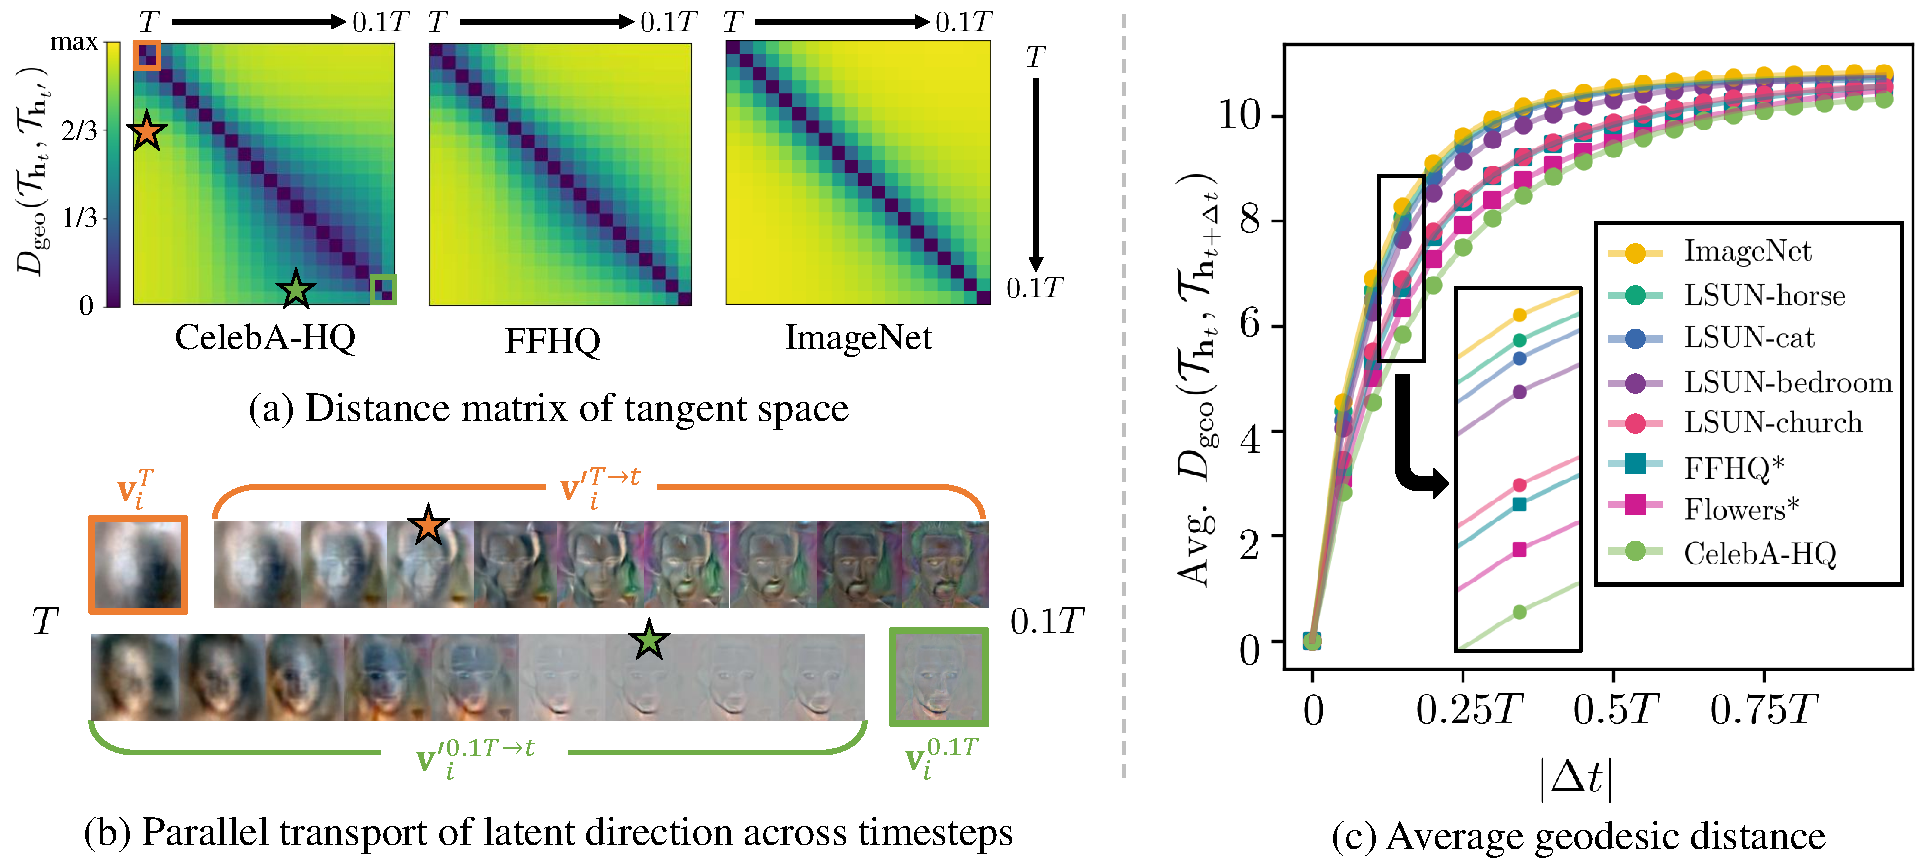
\includegraphics[width=1.0\linewidth]{figure/evolution-t.pdf}
%     \vspace{-1em}
%     \caption{
%     \textbf{Example images edited with global semantic directions.} Consistent semantic changes in two rows validate the global semantic direction. The attributes are manually interpreted because the directions are not supervised.}
%     \label{fig:global_basis_main}
% \end{figure}


% \begin{figure}[!t]
%     \centering
%     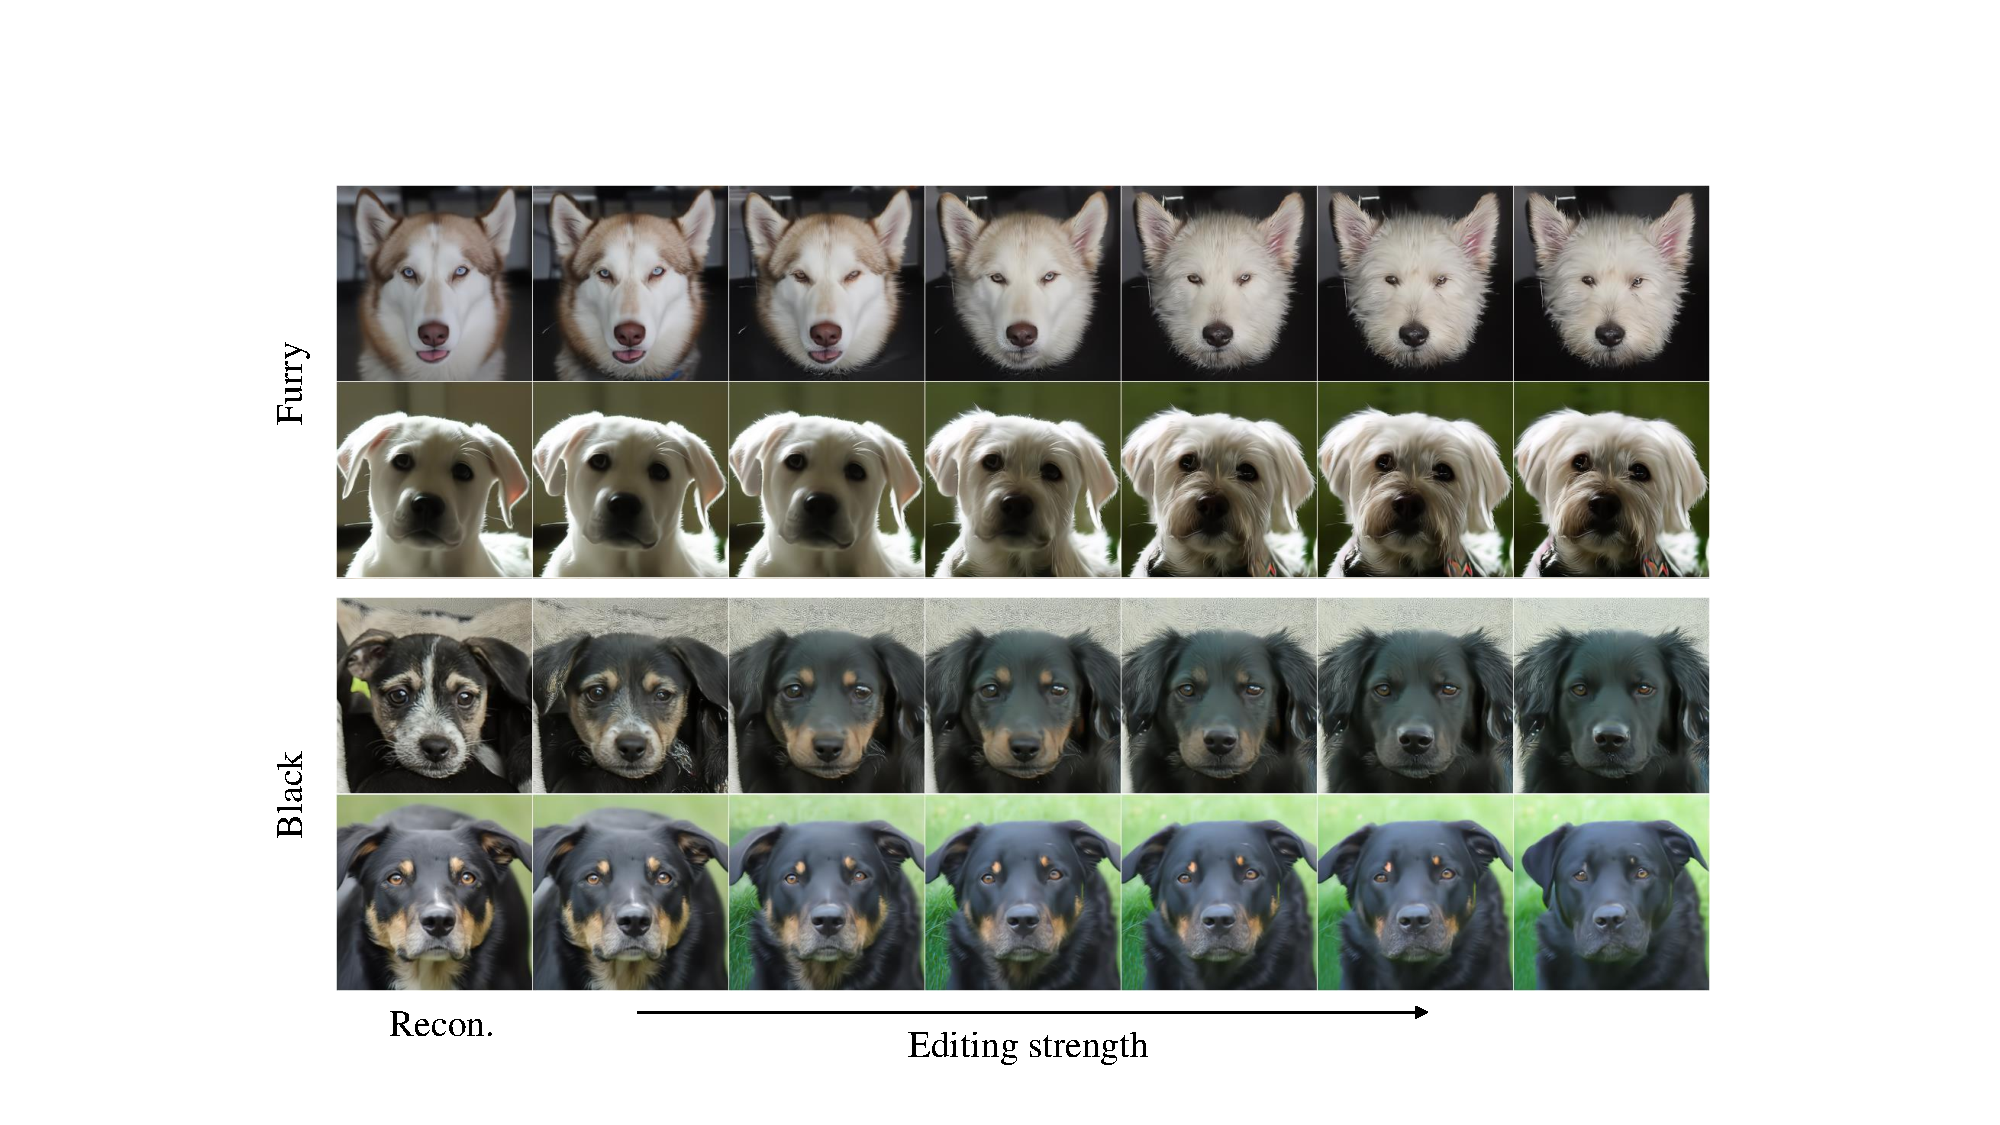
\includegraphics[width=1.0\linewidth]{figure/afhq_global.pdf}
%     \vspace{-1em}
%     \caption{
%     \textbf{Example images edited with global semantic directions.} Consistent semantic changes in two rows validate the global semantic direction. The attributes are manually interpreted because the directions are not supervised.}
%     \label{fig:global_basis_main}
% \end{figure}

% \begin{table}[t]
% \caption{Semantic path length for lerp, slerp, and geodesic paths in CelebA-HQ for DDPM++.}
% \label{tab:semantic_path_length}
% \vskip 0.15in
% \begin{center}
% \begin{small}
% % \begin{sc}
% \begin{tabular}{lc}
% \toprule
% Path & Semantic Path Length $(\mu \pm \sigma)$ \\
% \midrule
% lerp     & 10.29 $\pm$ 1.11 \\
% slerp    & 7.69 $\pm$ 0.87 \\
% geodesic & 5.98 $\pm$ 0.76 \\
% \bottomrule
% \end{tabular}
% % \end{sc}
% \end{small}
% \end{center}
% \vskip -0.1in
% \end{table}

% \begin{figure}[!t]
%     \centering
%     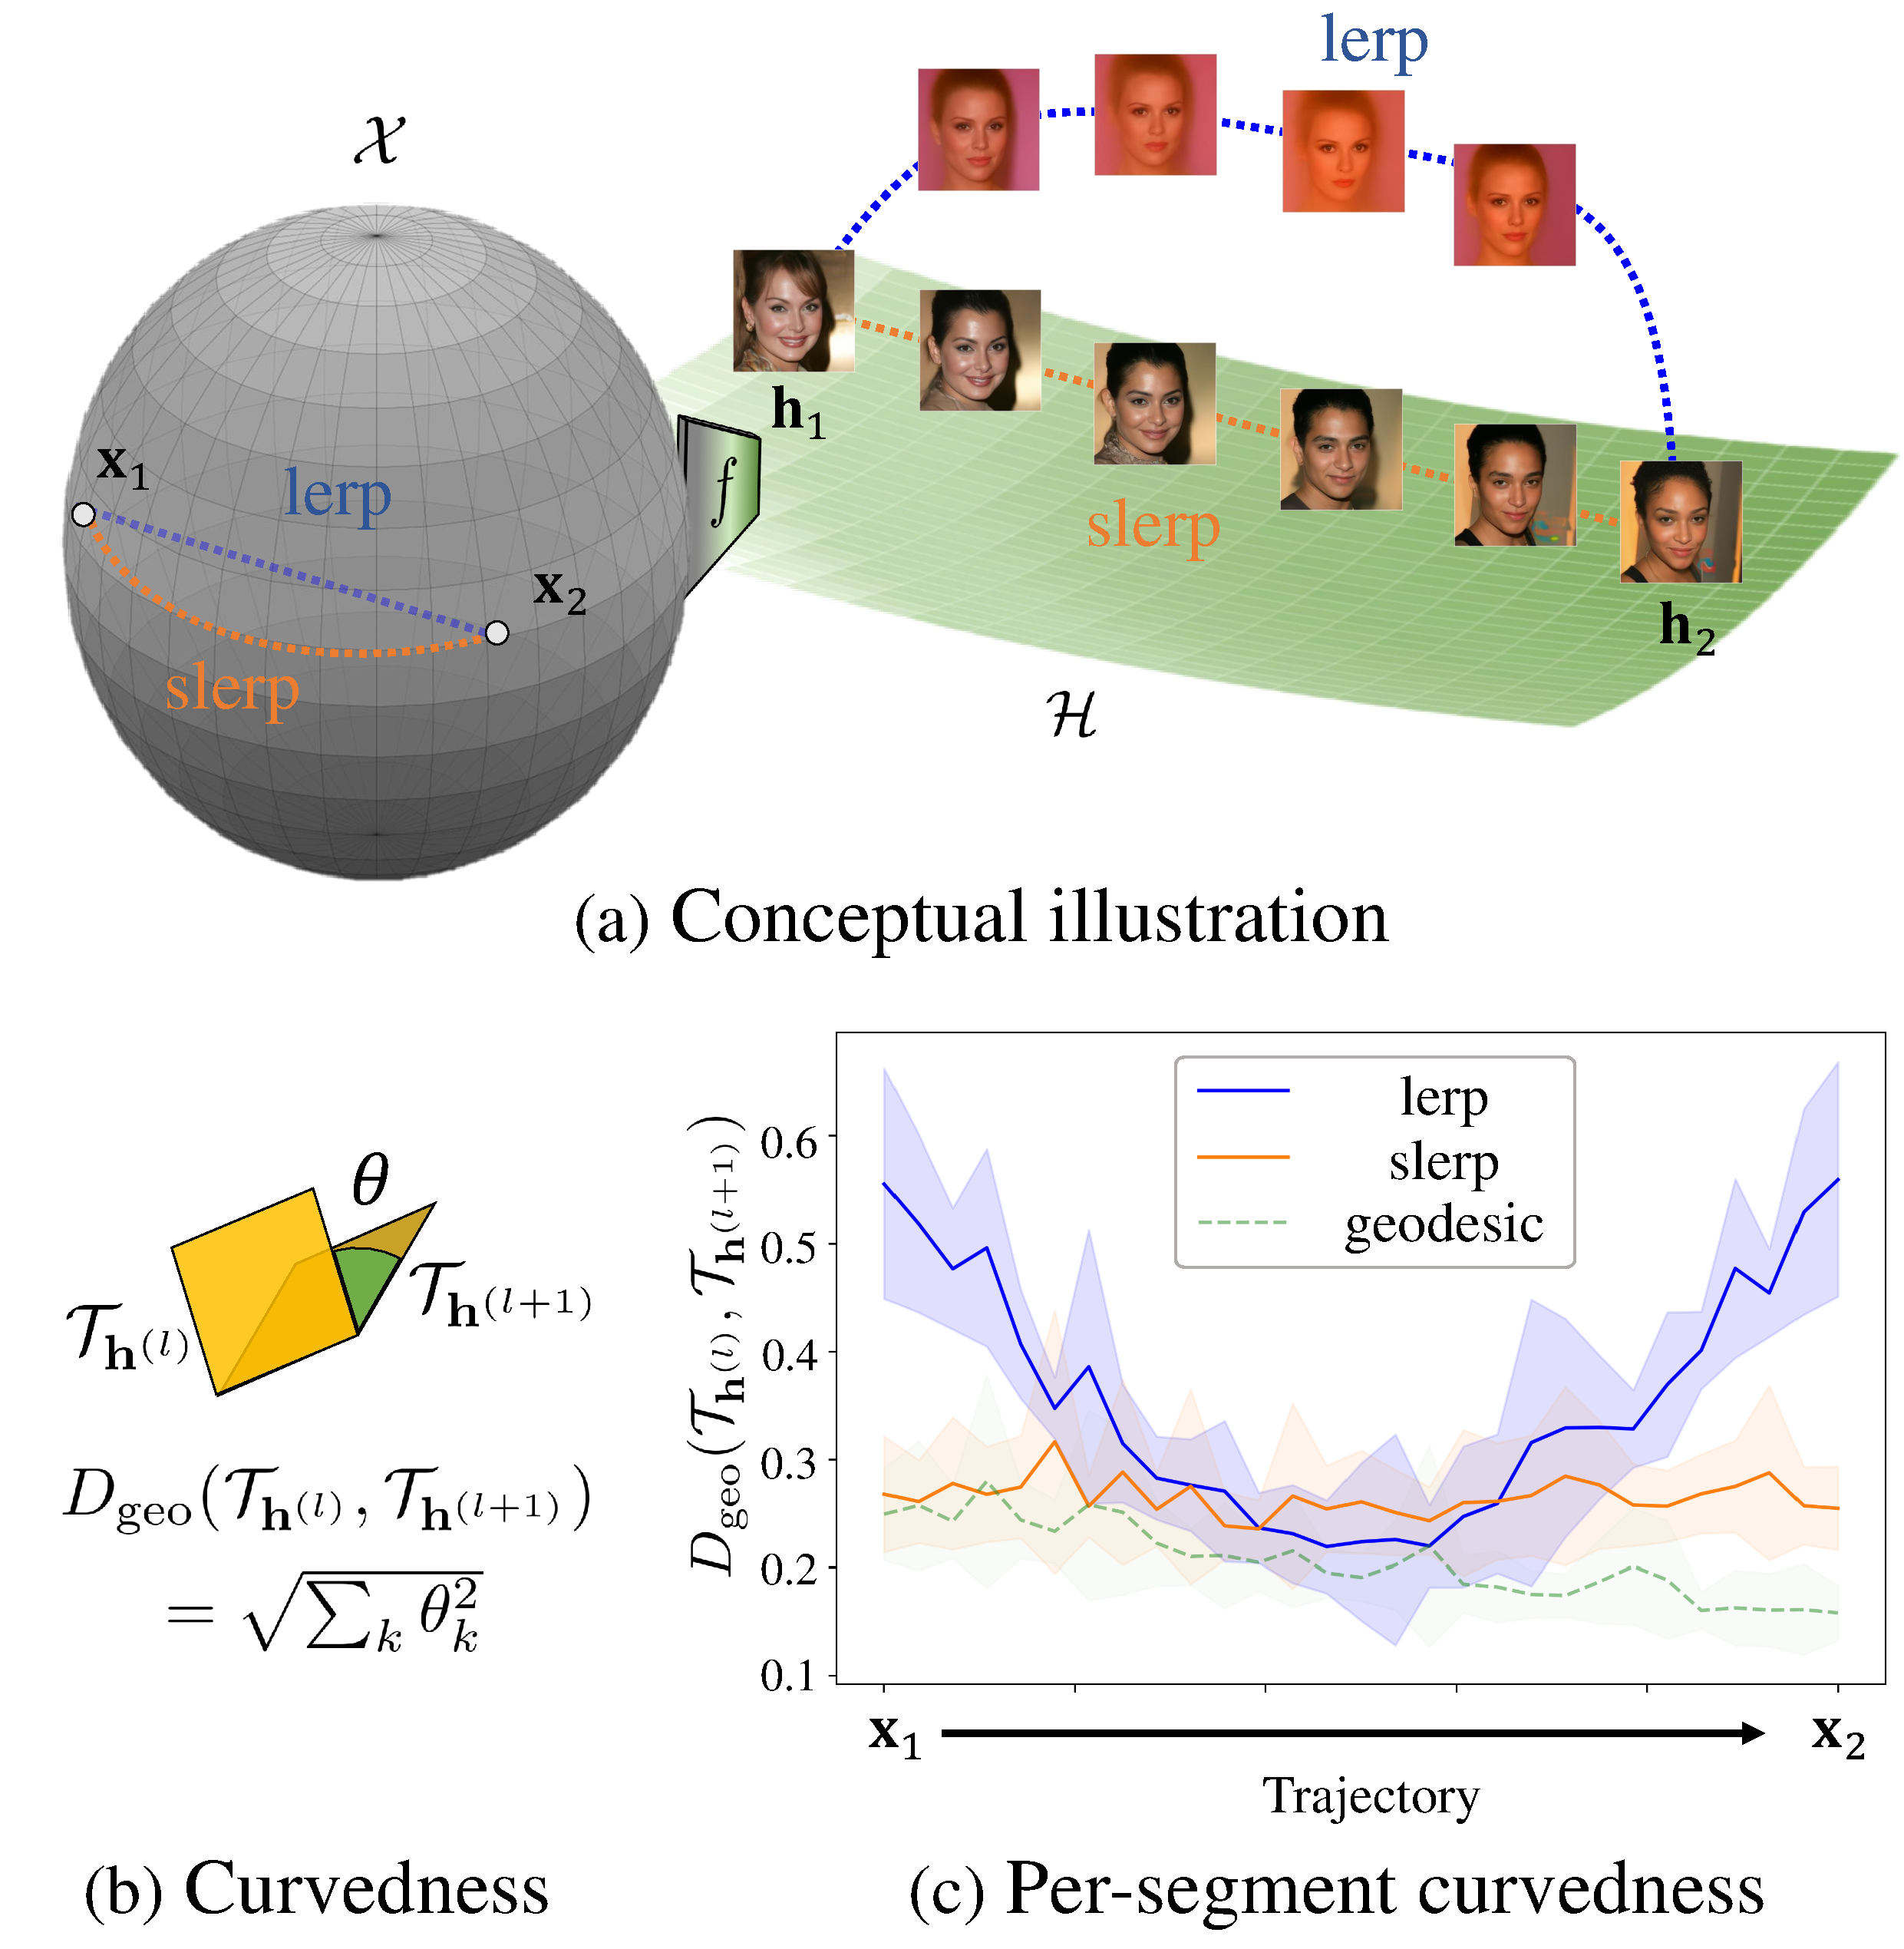
\includegraphics[width=1.0\linewidth]{./figure/slerp_lerp.pdf}
%     \vspace{-1em}
%     \caption{
%     \textbf{$\mathcal{X}$ is a curved manifold.}
%     (a) Conceptual illustration of a linear path (lerp) and a spherical path (slerp) on the manifolds.
%     (b) Curvedness of a line segment.
%     (c) Per-segment distribution of curvedness along different paths. The lerp paths roughly have higher curvedness than slerp and reach similar curvedness to slerp. The slerp paths are closer to the geodesic shooting paths. It implies that $\mathcal{X}$ is a curved manifold. The shades depict $\pm$ 0.5 standard deviation. We use 50 segments for each path between $\vx_1$ and $\vx_2$.
%     }
%     \label{fig:slerp_lerp}
% \end{figure}

% \subsection{Curved manifold of DMs} % \subsection{Indepth analysis on the latent space of DMs} 
% \label{sec:slerp}
% We present empirical grounds for the assumption in \sref{sec:method_local}: $\mathcal{X}$ is a curved manifold. Semantic path length between two points on a manifold is defined by the sum of the local warpage of the line segments which connects them along the manifold. We use \emph{geodesic metric}~\cite{choi2021not, ye2016schubert} to define the curvedness of a line segment $\{\vx^{(1)}, \vx^{(2)}\}$ as the angle between two tangent spaces centered at $\{\vh^{(1)}, \vh^{(2)}\}$: 
% \begin{equation}
% D_{\text{geo}}(\mathcal{T}_{\vh^{(1)}}, \mathcal{T}_{\vh^{(2)}}) = \sqrt{\sum_k \theta_k^2},
% \end{equation}
% where $\theta_k = \cos^{-1}(\sigma_k)$ denotes the $k$-th principle angle between $\mathcal{T}_{\vh^{(1)}}$ and $\mathcal{T}_{\vh^{(2)}}$.
% The angle is visualized in \fref{fig:slerp_lerp} (b). Then, the semantic path length becomes $\sum_l D_\text{geo}(\mathcal{T}_{\vh^{(l)}}, \mathcal{T}_{\vh^{(l+1)}})$, where $l$ denotes the segment index in the path. We set the number of segments to $30$.
% Then, the semantic path length increases as the path deviates further from the manifold.



% To verify the assumption, we compare the semantic path lengths of different paths, e.g., linear path, spherical path, and geodesic shooting path. 
% \fref{fig:slerp_lerp} (a) visualizes the manifold, linear path (lerp), and spherical path (slerp) and their corresponding path on $\mathcal{H}$ mapped by the function $f$. We computed the semantic path lengths for 50 randomly selected pairs of images. \tref{tab:semantic_path_length} shows that the semantic path length of slerp is smaller than lerp, indicating that the slerp path lies closer to the manifold than lerp, i.e., the manifold is curved. \fref{fig:slerp_lerp} (b) shows the distribution of the length of the segments along the path. Interestingly, the length of the lerp is high at the ends and shrinks to that of geodesics near the center. We suppose that the lerp path moves away from the original manifold and moves along another manifold.


% Our semantic path length resembles the perceptual path length (PPL, \citet{karras2019style}) regarding the summation along the interpolation path.
% PPL measures LPIPS \cite{zhang2018unreasonable} distance between resulting images along the path. Higher PPL between two latent variables indicates spikier interpolation of images accompanying artifacts. On the other hand, semantic path length measures how drastically the geometric structure changes between neighboring tangent spaces.





% \subsection{Ablation study}
% \subsection{Comparisons}
% \label{sec:ablation}
% We provide comparisons that include alternative approaches.
% First, we edit images by applying random directions instead of semantic latent directions. \fref{fig:ablation_random_dx_ours} shows that random directions seriously degrade the images. 
% This experiment validates the excellence of the latent directions found by our method.

% \paragraph{Random basis} 
% \paragraph{Zero-shot text-based editing} 

% \begin{figure}[!t]
%     \centering
%     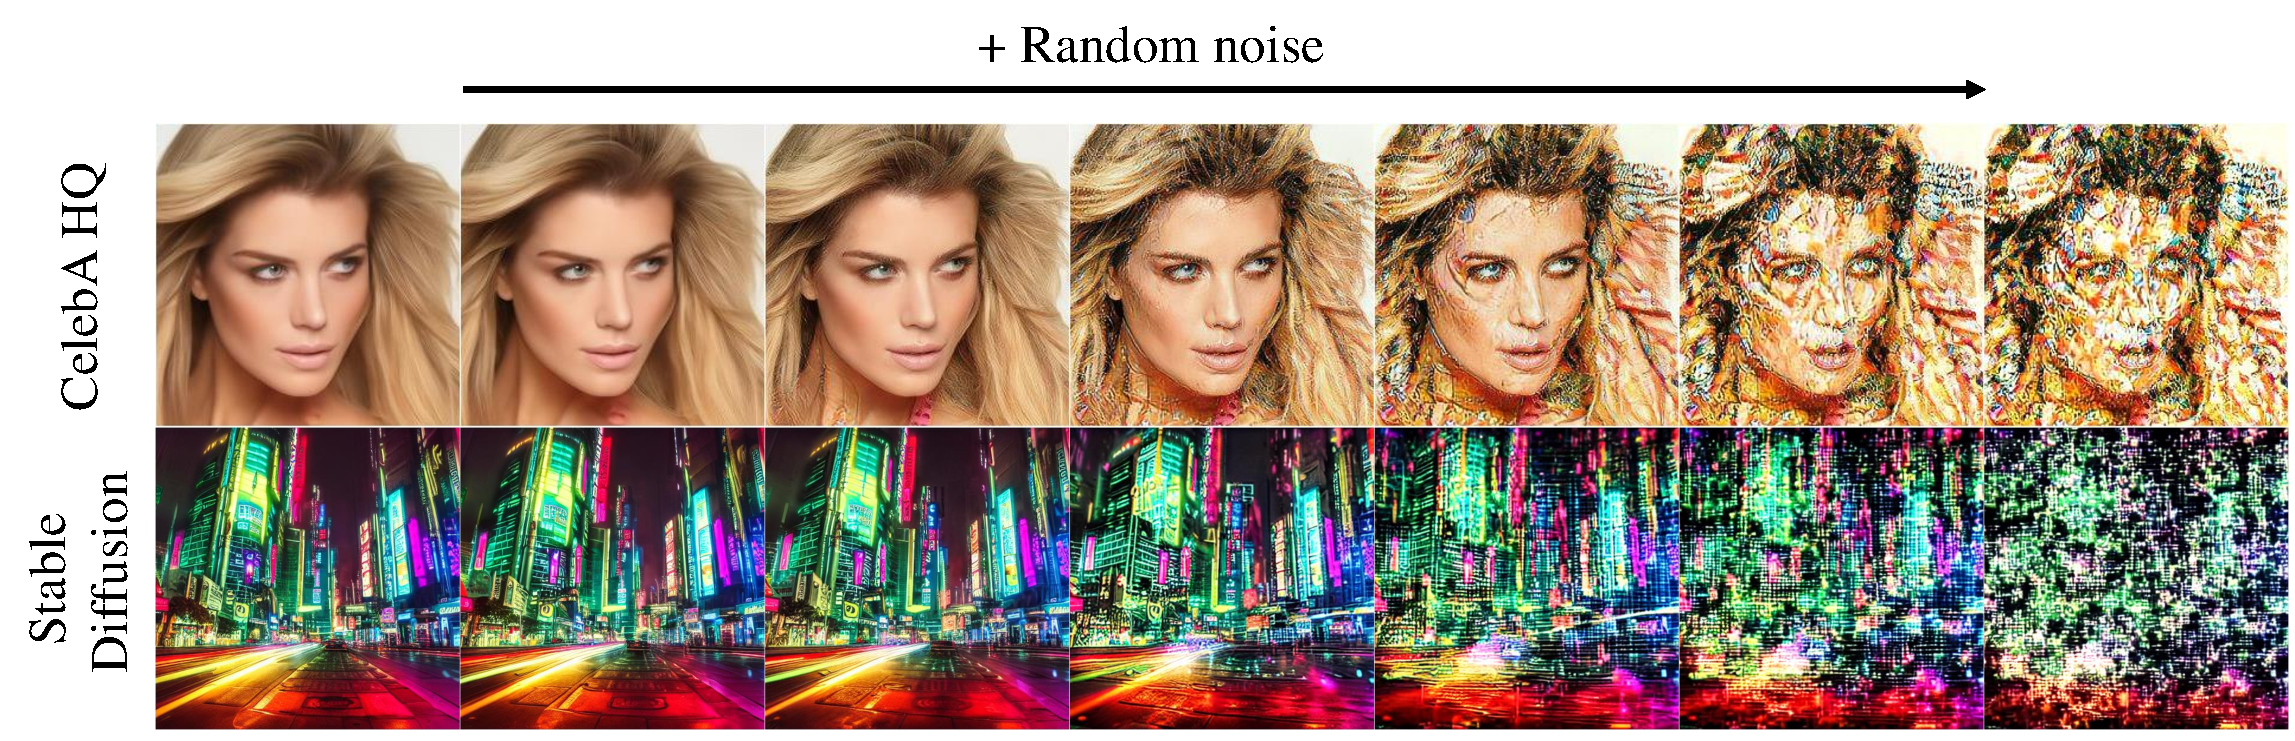
\includegraphics[width=1\linewidth]{figure/random.pdf}
%     \vspace{-1em}
%     \caption{
%     \textbf{Importance of the discovered semantic directions.} Adding random directions instead of semantic directions severely distorts the resulting images. 
%     }
%     \label{fig:ablation_random_dx_ours}
% \end{figure}

% \begin{figure}[!t]
%     \centering
%     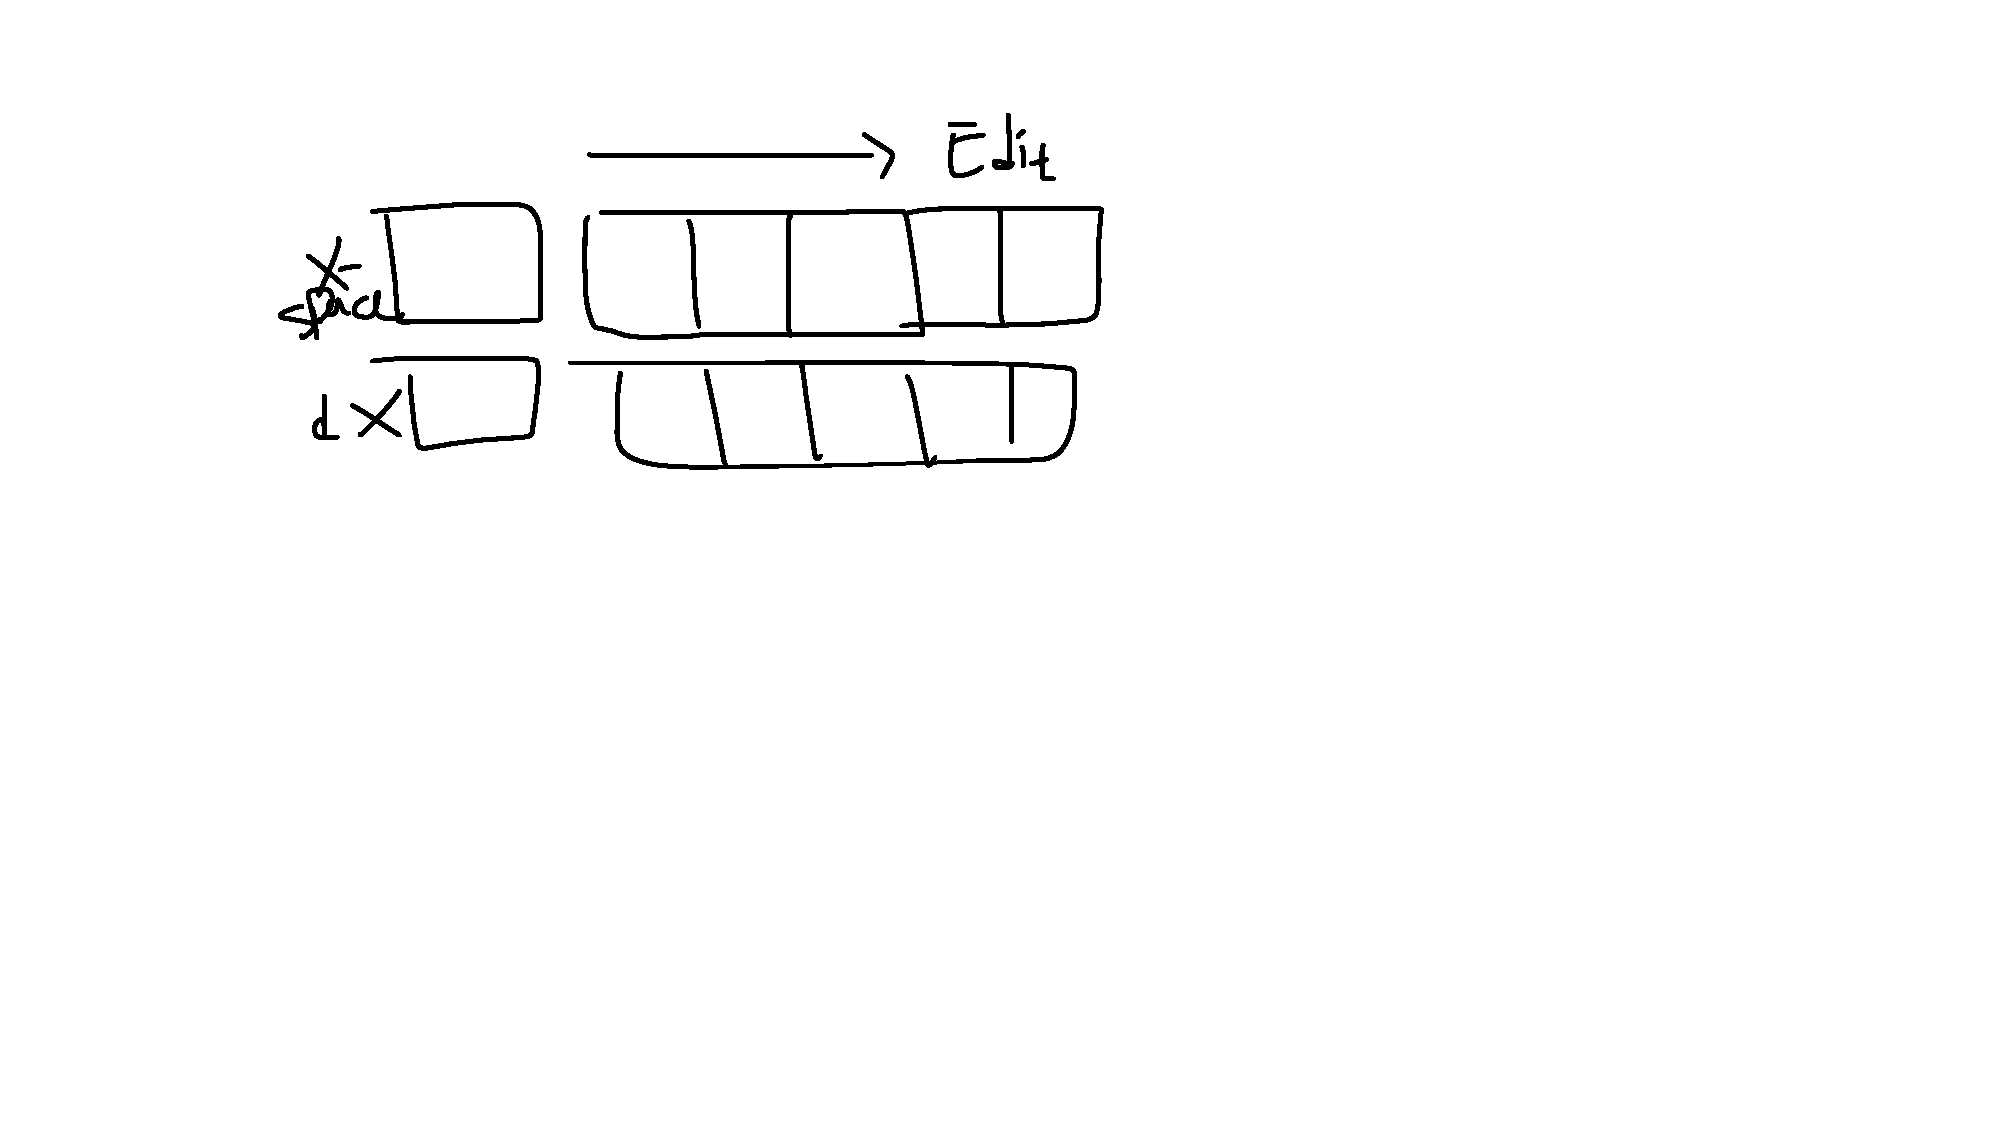
\includegraphics[width=1\linewidth]{figure/direct.pdf}
%     \vspace{-1em}
%     \caption{
%     \textbf{Importance of the normalization in \eref{eq:cpc}.} Removing the normalization leads to excessive saturation.
%     }
%     \label{fig:ablation_direct_dx_ours}
% \end{figure}

% \fref{fig:ablation_direct_dx_ours} demonstrates the necessity of normalization in \eref{eq:cpc}. While our full method produces plausible edited images even with extreme changes, removing the normalization leads to excessive saturation.


% \begin{figure}[!t]
%     \centering
%     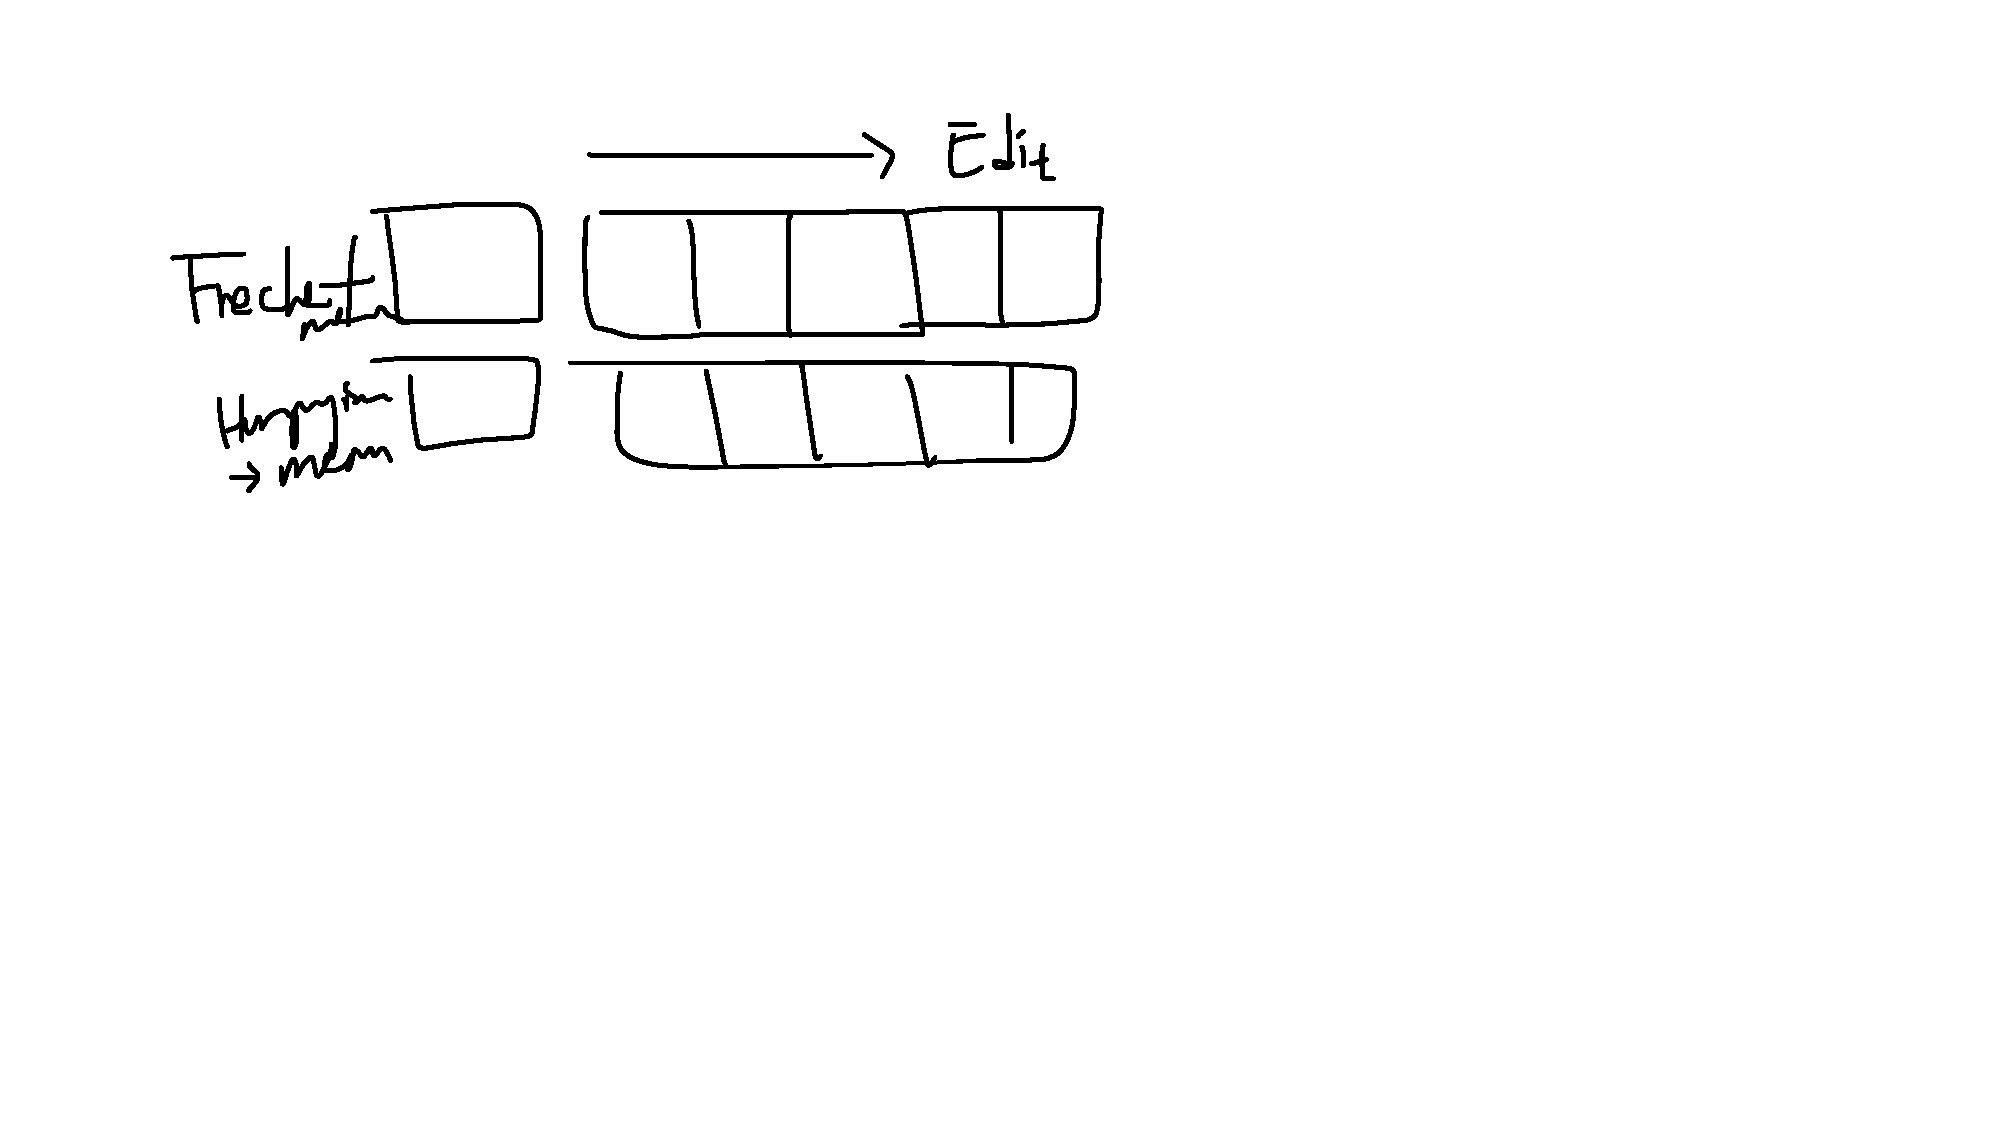
\includegraphics[width=1.\linewidth]{figure/global_ablation.pdf}
%     \vspace{-1em}
%     \caption{
%     \textbf{Inferiority of GANSpace on $\mathcal{H}$.} The GANSpace directions accompany severe distortion or entanglement while somewhat altering the attributes such as expression, rotation, and age.}
%     \vspace{-1em}
%     \label{fig:global_ablation}
% \end{figure}

% \subsection{Comparison to other editing methods}
% \label{sec:comparison}
% As we introduce the first unsupervised editing in DMs, we compare our method with GANSpace \cite{harkonen2020ganspace} considering the mapping from $\mathcal{X}$ to $\mathcal{H}$ instead of $\mathcal{Z}$ to $\mathcal{W}$ in GANs. Accordingly, we find directions in $\mathcal{H}$ using PCA. \fref{fig:ganspace} shows their effects: they somewhat alter the attributes but accompany severe distortion or entanglement. On the contrary, our method finds the directions with the largest changes in $\mathcal{H}$ considering the geometrical structure leading to decent manipulation as shown in earlier results. \aref{appendixsec:comparison} describes more details for GANSpace.


% \vspace{-1em}